% !TEX root = /Users/jonasfrugte/Desktop/Research_Project/fisher_calc_weak_lensing/paper/paper_draft.tex
\documentclass[11pt]{article} % Choose a document class, like 'article', 'report', or 'revtex4-2' for scientific papers

% Packages to enhance functionality
\usepackage[utf8]{inputenc}   % Allows UTF-8 character encoding
\usepackage{amsmath}          % For advanced math typesetting
\usepackage{amssymb}          % Additional math symbols
\usepackage{graphicx}         % For including images
\usepackage{hyperref}         % For hyperlinks in the document
\usepackage{geometry}         % For setting up page geometry
\geometry{margin=1in}         % 1-inch margins all around
\usepackage{authblk}          % For author affiliations
\usepackage{siunitx}          % For consistent typesetting of units
\usepackage{subcaption}       % For subfigures within a figure
\usepackage{float}            % To control float positioning (e.g., figures/tables)
\usepackage{enumitem}         % Better control over list formatting
\usepackage{tocloft}
\usepackage{tikz}
\usepackage{tikz-3dplot}
\usetikzlibrary{shapes.geometric, arrows, backgrounds}
\usepackage{empheq}
\usepackage{booktabs}
\usepackage{authblk}
\usepackage{multirow} % needed for merging cells vertically
\usepackage{booktabs}


\usepackage{listings}
\usepackage{xcolor} % For color customization (optional)

\usepackage[backend=biber, style=numeric]{biblatex}
\addbibresource{/Users/jonasfrugte/Desktop/Research_Project/fisher_calc_weak_lensing/paper/sources.bib}

\lstset{
    language=Python,
    basicstyle=\ttfamily\small,
    keywordstyle=\color{blue}\bfseries,
    stringstyle=\color{red},
    commentstyle=\color{gray}\itshape,
    showstringspaces=false,
    frame=single, % Adds a frame around the code
    breaklines=true % Wrap long lines
}

% some custom commands that should've already been in latex by default
\DeclareRobustCommand{\d}{\ifmmode\text{d}\else d\fi}
\DeclareRobustCommand{\Cov}{\ifmmode\text{Cov}\else d\fi}
\DeclareRobustCommand{\CMB}{\ifmmode\text{CMB}\else d\fi}
\DeclareRobustCommand{\gal}{\ifmmode\text{gal}\else d\fi}

\newcommand{\br}[1]{\ensuremath{\left( #1 \right)}}
\newcommand{\sbr}[1]{\ensuremath{\left[ #1 \right]}}

\setlength{\cftbeforesecskip}{5pt}

% Additional customizations (optional)
\setlength{\parindent}{0pt}   % No paragraph indentation
\setlength{\parskip}{1em}     % Add space between paragraphs

\title{\huge \textbf{Parameter Forecasts From CMB Lensing and Galaxy Lensing Power- and Bispectra}}

\author[1]{\textbf{Jonas Frugte}}
\author[2]{\textbf{P. Daniel Meerburg}}

\affil[1]{Independent Researcher, The Netherlands}
\affil[2]{Van Swinderen Institute for Particle Physics and Gravity, University of Groningen, Nijenborgh 4, 9747 AG Groningen, The Netherlands}
\affil[ ]{}
\affil[ ]{\textit{E-mail:} \texttt{jonasfrugte@gmail.com}}
 % Removes the default date

\begin{document}
\maketitle

% \textbf{
%     \huge \noindent 
%     Parameter Forecasts From CMB $\times$ Galaxy Lensing Powerspectra $\times$ Bispectra
%     \vspace{0.5cm}
%     \\
%     \normalsize
%     Jonas Frugte, Daan Meerburg\\
%     20 February 2025
%     }\\
% \vspace{0.5cm}

\begin{center}
    \textbf{NB: Currently still in draft.}
\end{center}
\hrule

\begin{abstract}
    % Weak gravitational lensing of the Cosmic Microwave Background (CMB) and distant galaxies provides a powerful probe of the large-scale structure and cosmic expansion history. Upcoming Stage-IV surveys like the Simons Observatory, CMB-S4, LSST, and Euclid promise unprecedented precision, motivating detailed forecasts of their constraining power. While lensing power spectra are standard cosmological tools, non-Gaussianities induced by structure formation encode additional information in the bispectrum. In this work, we perform a comprehensive Fisher matrix forecast to quantify the detectability of these signals and the cosmological constraints achievable by combining power spectrum and bispectrum measurements from both CMB lensing and galaxy shear, including their cross-correlations. We model Stage-IV-like experimental specifications and forecast constraints on the standard $\Lambda$CDM parameters, the sum of neutrino masses ($\Sigma m_\nu$), and the dark energy equation of state ($w_0$). We demonstrate that incorporating bispectra significantly enhances constraints, reducing marginalized parameter uncertainties by up to $\sim \texttt{X}\%$ compared to power spectra alone. We project competitive constraints, including $\sigma(H_0) = \texttt{X.X~km/s/Mpc}$, $\sigma(\sigma_8) = \texttt{X.XXX}$, and $\sigma(\Sigma m_\nu) = \texttt{X.XX~eV}$.
    \end{abstract}
\pagebreak
%\tableofcontents

% \section{Conventions}
% Use $\mathbf k$ for wave numbers (Fourier space), $l$ for multipole moments, $m$ for magnetic quantum number. $P^{XY}(k, \eta, \eta')$ and $B^{XYZ}(k_1,k_2,k_3, \eta_1, \eta_2, \eta_3)$ correspond to bi and power spectra of fields $X$, $Y$, and $Z$ in Fourier space. $P_l^{XY}(\eta,\eta')$ and $B_{l_1l_2l_3}^{XYZ}(\eta_1, \eta_2, \eta_3)$ correspond to the multipole moments of the bi and power spectra of fields $X$, $Y$, and $Z$. If all times are the same we may instead write only one time argument and if the time is current time then we omit the time argument entirely. In other words,
% $$
% P_l^{XY}(\eta):=P_l^{XY}(\eta,\eta), \quad P_l^{XY}:=P_l^{XY}(\eta_{\text{current}}), \quad \text{similarly for all other spectra}.
% $$
% If both fields are the same, we may only denote one field, e.g. 
% $$
% P_l^{X}(\eta) := P_l^{XX}(\eta).
% $$

% Our Fourier convention is
% \begin{align}
%     &\text{Forward Transform:} & \quad \tilde{f}(k) &= \int_{-\infty}^{\infty} f(x) \, e^{-i k x} \, dx\\
%     &\text{Inverse Transform:} & \quad f(x) &= \frac{1}{2\pi} \int_{-\infty}^{\infty} \tilde{f}(k) \, e^{i k x} \, dk
% \end{align}
% we choose this convention because it is in line with the convention used in the CAMB source code. We work in natural units where $c=1$.

\section{Introduction}

Weak lensing has been used as a probe to constrain cosmological parameters since the 2000's \cite{kilbinger2015cosmology,Bacon2000,Kaiser2000,Waerbeke2000,Bartelmann2001}. A range of upcoming surveys, such as the survey by the Simons Observatory (SO) \cite{Ade2019}, the Legacy Survey of Space and Time (LSST) \cite{Ivezic2019}, and Euclid \cite{Laureijs2011} aim to measure weak lensing of the CMB and of galaxies. They will do so much more accurately than previous surveys, enabling tighter constraints on parameters and progressing our understanding of physics as a whole. Typically, the main value of interest is the power spectrum (or equivalently, two point function) of the lensing potential. This can be measured in terms of the lensing convergence $\kappa$, lensing shear $\gamma$, or lensing potential $\psi$. In the weak lensing regime they all contain the same amount of information and can be easily converted into one another, see section \ref{sec:weaklensstats}. For the CMB the lensing potential is generally measured directly \cite{Planck2018Lensing}, while with galaxies one instead measures the shear, as this can be deduced from the ellipiticity distribution of the observed galaxies \cite{HoekstraJain2008}.

Even with Gaussian initial conditions, there are significant amounts of non-Gaussianity in the weak lensing signal, especially in galaxy lensing due to it being a probe of the more recent distribution of matter \cite{Bernardeau1997,Takada2003}. In addition to looking at the power spectrum, a natural next step is thus to measure the lensing bispectrum. This has already been done for signals from galaxies \cite{vanWaerbeke2002}, but no proper detection has been done of the CMB lensing bispectrum. Upcoming surveys such as the ones mentioned earlier may detect this signal. Therefore it is relevant to know the detectability of, and parameter constraints possible from, all 4 signals: CMB lensing power- and bispectra and galaxy lensing power- and bispectra. Notably, this includes looking at cross correlation as well. 

In this article we aim to answer this question in the context of experimental parameters similar to those of next generation surveys such as mentioned earlier. We are especially interested in seeing if approximate parameter degeneracies can be broken by combining all data. Calculating the covariance matrix of unbiased optimal estimators of the cosmological parameters can be done by combining cosmological simulations (in our case we use the CAMB package \cite{Lewis2000}) with a Fisher matrix analysis. See figure \ref{fig:flowchart} for an overview of the calculation done in this paper. The parameters looked at are the Hubble constant, $H_0$, physical baryon density, $\Omega_b h^2$, physical cold dark matter density, $\Omega_c h^2$, scalar spectral index, $n_s$, amplitude of primordial scalar fluctuations, $A_s$, sum of neutrino masses $\sum m_\nu$, and dark energy equation of state parameter, $w_0$. Though, we will find that some of the parameters are poorly constrained even when combining all 4 signals and thus omit them from the analysis in the results. As a secondary purpose, this paper also includes a derivation for the Fisher matrix formalism in the non-trivial context of bispectra with multiple tracers. The final formula can already be found in the literature (see e.g.\ the appendix of \cite{Kalaja_2021}), but the authors of this paper were not able to find a derivation and hence included it.

The structure of this paper is as follows: we first review the theory of weak lensing and weak lensing statistics in sections \ref{sec:weaklensing} and \ref{sec:weaklensstats}. We then provide technical details of the calculation in section \ref{sec:calcdetails}, such as choices for noise and numerical approximations made in the code. In section \ref{sec:results} we present the results, consisting of signal to noise ratios and parameter constraints for different combinations of the CMB and galaxy lensing power- and bispectra. We conclude in section \ref{sec:discussion}. Appendix \ref{sec:fisher} contains a short review of the Fisher matrix formalism and gives a technical derivation of the formula used to calculate each Fisher matrix element in the case of bispectra measurements with multiple tracers. Finally, appendix \ref{sec:shear} explains how to relate the shear to the lensing potential in spherical harmonic space.

All code written for this project is uploaded on github at \url{https://github.com/Jonas-Frugte/fisher_calc_weak_lensing}.



\begin{figure}[h!]
    \centering
    
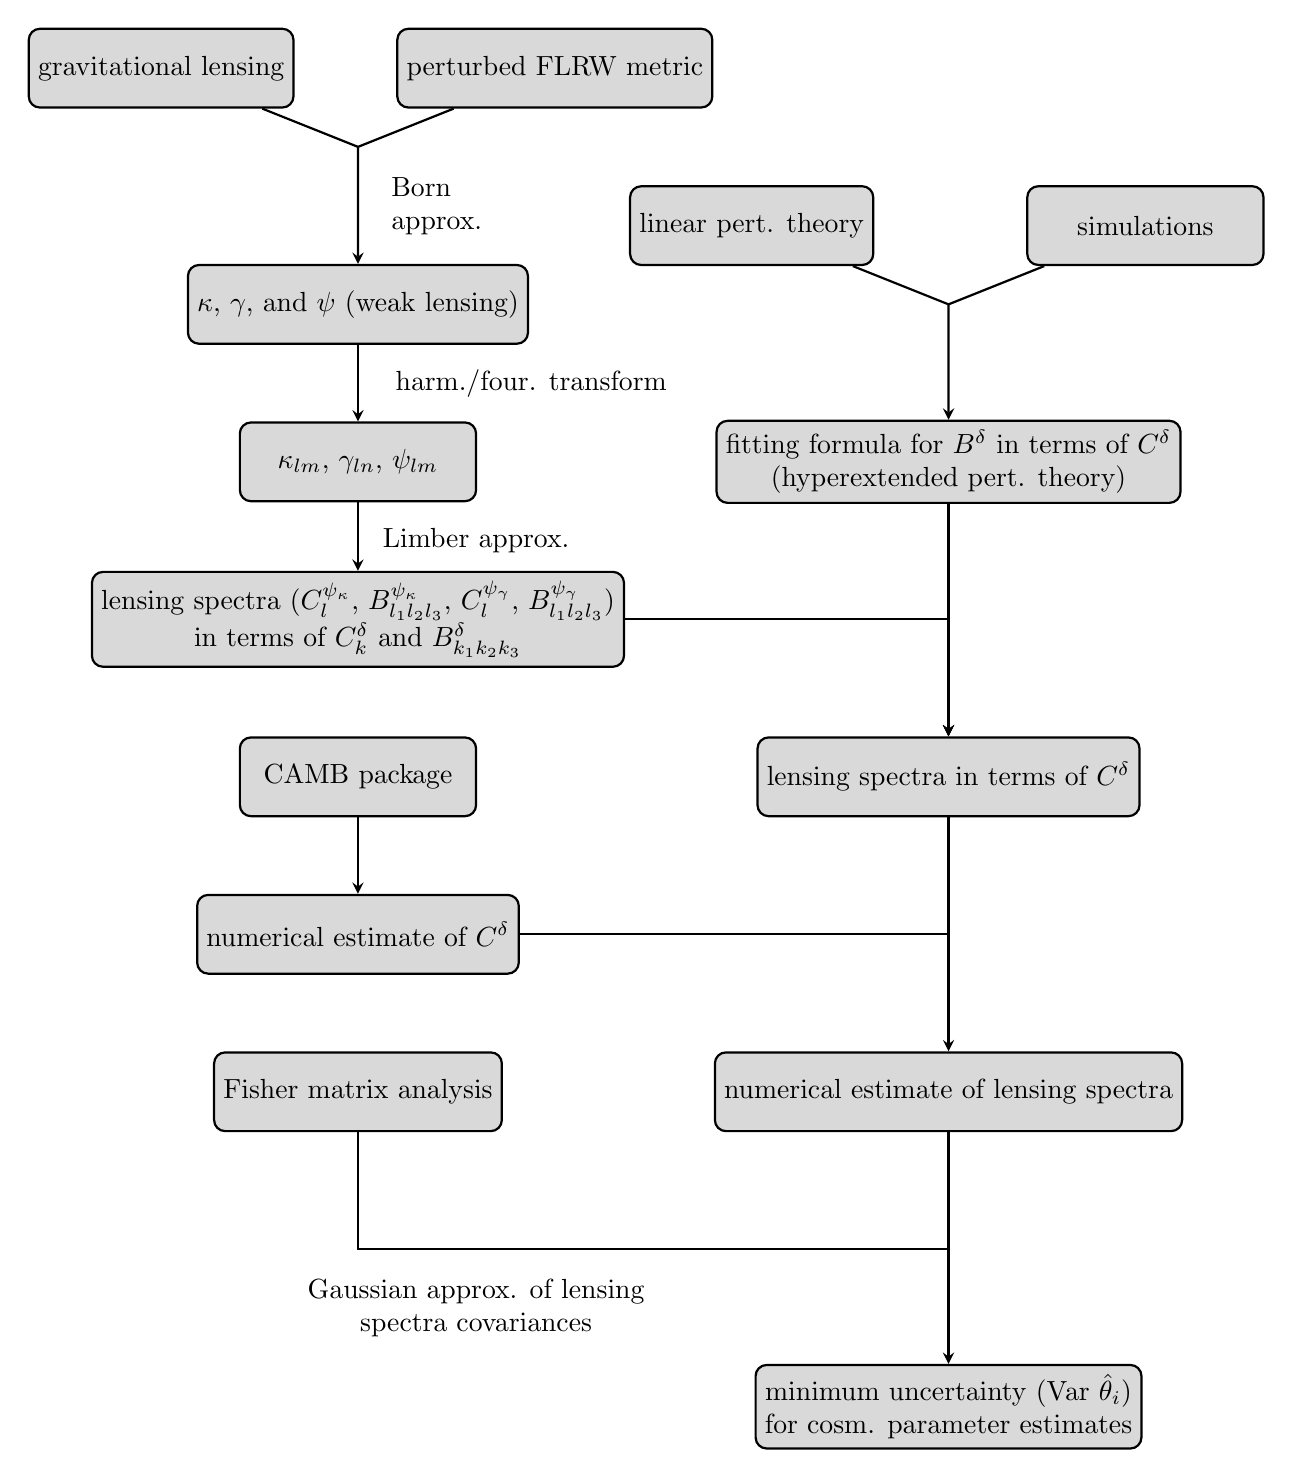
\begin{tikzpicture}[node distance=2cm, thick, background grid/.style={help lines, color=gray!30, step=0.5cm}]
    % Background grid
    % \begin{scope}[background grid]
    %     \draw[background grid] (0, 0) grid (15, 15);
    % \end{scope}

    % Define styles for boxes and arrows
    \tikzstyle{process} = [rectangle, rounded corners, minimum width=3cm, minimum height=1cm, text centered, draw=black, fill=gray!30]
    \tikzstyle{arrow} = [thick,->,>=stealth]
    \tikzstyle{line} = [thick,-]
    \tikzstyle{curve arrow} = [thick,->,>=stealth, looseness=1.2, bend left=30]

    % boxes
    \node (lensing) [process] at (0, 15) {gravitational lensing};
    \node (FLRW) [process] at (5, 15) {perturbed FLRW metric};
    \node (weak) [process] at (2.5, 12) {$\kappa$, $\gamma$, and $\psi$ (weak lensing)};
    \node (weakharm) [process] at (2.5, 10) {$\kappa_{lm}$, $\gamma_{ln}$, $\psi_{lm}$};
    \node (lensstats) [process, align=center] at (2.5, 8) {
        lensing spectra ($C^{\psi_\kappa}_l$, $B^{\psi_\kappa}_{l_1l_2l_3}$, $C^{\psi_\gamma}_l$, $B^{\psi_\gamma}_{l_1l_2l_3}$)\\ in terms of $C^\delta_{k}$ and $B^\delta_{k_1k_2k_3}$
        };
    \node (linearpert) [process] at (7.5, 13) {linear pert. theory};
    \node (sim) [process] at (12.5, 13) {simulations};
    \node (hyperextendedpert) [process, align=center] at (10, 10) {fitting formula for $B^\delta$ in terms of $C^\delta$ \\ (hyperextended pert. theory)};
    \node (lensspectermsofmatterpower) [process] at (10, 6) {lensing spectra in terms of $C^\delta$};
    \node (camb) [process] at (2.5, 6) {CAMB package};
    \node (numericalmps) [process] at (2.5, 4) {numerical estimate of $C^\delta$};
    \node (numericallensingspectra) [process] at (10, 2) {numerical estimate of lensing spectra};
    \node (fisher) [process] at (2.5, 2) {Fisher matrix analysis};
    \node (end) [process, align=center] at (10, -2) {minimum uncertainty ($\text{Var }\hat\theta_i$) \\ for cosm. parameter estimates};

    % extra
    \node [align=left] at (3.5, 13.25) {Born \\ approx.};
    \node [align=left] at (4.7, 11) {harm./four. transform};
    \node [align=left] at (4, 9) {Limber approx.};
    \node [align=center] at (4, -0.75) {Gaussian approx. of lensing \\ spectra covariances};

    % Arrows
    \draw [arrow] (FLRW) -- (2.5, 14) -- (weak);
    \draw [line] (lensing) -- (2.5, 14);
    \draw [arrow] (weak) -- (weakharm);
    \draw [arrow] (weakharm) -- (lensstats);
    \draw [arrow] (linearpert) -- (10, 12) -- (hyperextendedpert);
    \draw [line] (sim) -- (10, 12);
    \draw [arrow] (camb) -- (numericalmps);
    \draw [arrow] (hyperextendedpert) -- (10, 8) -- (lensspectermsofmatterpower);
    \draw [line] (lensstats) -- (10, 8);
    \draw [arrow] (hyperextendedpert) -- (10, 8) -- (lensspectermsofmatterpower);
    \draw [arrow] (hyperextendedpert) -- (10, 8) -- (lensspectermsofmatterpower);
    \draw [arrow] (lensspectermsofmatterpower) -- (10, 4) -- (numericallensingspectra);
    \draw [line] (numericalmps) -- (10, 4);
    \draw [arrow] (numericallensingspectra) -- (10, 0) -- (end);
    \draw [line] (fisher) -- (2.5, 0) -- (10, 0);
\end{tikzpicture}
    \caption{Flowchart of steps involved in calculating the minimum error/uncertainty in cosmological parameter estimates using convergence and shear power- and bi-spectra.}
    \label{fig:flowchart}
\end{figure}

\section{Theory}
\subsection{Weak lensing spectra}
Radiation from cosmological objects is distorted due to gravitational lensing. In the vast majority of cases this lensing is a relatively weak effect and is thus referred to as weak lensing. Weak lensing is quantified through the deflection field $\mathbf d(\hat {\mathbf n})$ which equals the difference between the observed angle of a point on the sky and the true (unlensed) angle. This field is the gradient of the lensing potential $\psi(\hat {\mathbf n})$ given as a weighted integral over the mass distribution along the line of sight between earth and the observed point.

In the case of CMB surveys, lensing alters the statistical properties of the temperature and polarization fields and can thus be calculated by comparing to the expected unlensed signal, see e.g. \cite{cmblensingestimator}. In galaxy surveys, lensing alters the ellipiticities of observed galaxies. If a large enough number of galaxies are observed, this effect can be seperated from the intrinsic ellipiticities of the galaxies and thus the lensing potential can be estimated.

To constrain cosmological parameters we can then look at the lensing potential of the CMB, $\psi_\CMB$, and of galaxy surveys, $\psi_\gal$. These are directly related to the matter power and bispectra as
\begin{empheq}[box=\fbox]{align*}
    C^{\psi_X\psi_Y}_l
    & = \frac{9}{l^4}\Omega_m^2H_0^4\int_0^{\chi_*} \chi^2 \d\chi a(\eta_0-\chi)^{-2}W_X(\chi)W_Y(\chi)C^\delta(l/\chi,\eta_0-\chi),\\
    B^{\psi_X\psi_Y\psi_Z}_{l_1l_2l_3} &= \sqrt{\frac{(2l_1 + 1)(2l_2 + 1)(2l_3 + 1)}{4\pi}} \begin{pmatrix} l_1 & l_2 & l_3 \\ 0 & 0 & 0 \end{pmatrix} \frac{27}{l_1^2l_2^2l_3^2}\Omega_m^3H_0^6\\
    & \quad \times \int \chi^2\d \chi a(\eta_0-\chi)^{-3}W_X(\chi)W_Y(\chi)W_Z(\chi)  B^\delta(\{l_i/\chi\}, \eta_0-\chi),
\end{empheq}
with $X, Y, Z \in \{\CMB, \gal\}$. $\Omega_m$ is the present day matter density parameter, $H_0$ is the present day Hubble constant, $a(\eta)$ is the scale factor, $\eta_0$ is the conformal time today, $\chi$ is the comoving radial distance, $\chi_*$ the distance to surface of last scattering, $P^\delta(k, \eta)$ the matter power spectrum, $B^\delta(k_1, k_2, k_3, \eta)$ the matter bispectrum, $W_X(\chi)$ the window function, and
$$
\begin{pmatrix}
    l_1&l_2&l_3 \\ m_1 & m_2 & m_3
\end{pmatrix}
$$ 
the Wigner 3-j symbol. The only factor that differs between CMB and galaxy lensing is the window function, defined as
\begin{equation*}
    W_X(\chi) = \int_\chi^{\infty}\d\chi' p_X(\chi')\frac{\chi'-\chi}{\chi'\chi},
\end{equation*}
with $p_X$ the radius distribution of the radiation source. For the CMB we take $p(\chi) = \delta(\chi - \chi_*)$. Notice that we can also look at cross correlation between CMB and galaxy lensing.

For a derivation of the lensing potential and its power- and bispectra, see appendices \ref{sec:weaklensing} and \ref{sec:weaklensstats}.

\subsection{Nonlinear matter bispectrum}
Determining the nonlinear matter powerspectrum can be done using numerical codes such as CAMB. The nonlinear matter bispectrum was calculated from the powerspectrum using a fitting formula based on perturbation theory in \cite{bispfit}. It is given by
\begin{equation}
    B^\delta(k_1, k_2, k_3, \chi) = 2 F_2(k_1, k_2, z) C^\delta(k_1, z) C^\delta(k_2, z) + \text{2 perm.}
\end{equation}
where \( C^\delta \) is the nonlinear matter power spectrum\footnote{Compare to the tree level bispectrum where we instead use the linear powerspectrum.}, and the kernel \( F_2 \) is modified from the tree level result with factors \( a(k, z) \), \( b(k, z) \), and \( c(k, z) \):
\begin{equation}
    F_2(k_1, k_2, z) = \frac{5}{7} a(k_1, z) a(k_2, z) + \frac{k_1^2 + k_2^2}{2 k_1 k_2} b(k_1, z) b(k_2, z) \cos \theta + \frac{2}{7} c(k_1, z) c(k_2, z) \cos^2 \theta.
\end{equation}
They are defined as:
\begin{equation}
    a(k, z) = \frac{1 + \sigma_8^{a_6}(z) \sqrt{0.7} Q(n_{\text{eff}}) (q^{a_1})^{n_{\text{eff}} + a_2}}{1 + (q^{a_1})^{n_{\text{eff}} + a_2}},
\end{equation}
\begin{equation}
    b(k, z) = \frac{1 + 0.2 a_3 (n_{\text{eff}} + 3) (q^{a_7})^{n_{\text{eff}} + 3 + a_8}}{1 + (q^{a_5})^{n_{\text{eff}} + 3.5 + a_8}},
\end{equation}
\begin{equation}
    c(k, z) = \frac{1 + \left[ \frac{4.5 a_4}{1.5 + (n_{\text{eff}} + 3)^4} \right] (q^{a_5})^{n_{\text{eff}} + 3 + a_9}}{1 + (q^{a_5})^{n_{\text{eff}} + 3.5 + a_9}}.
\end{equation}
Here, \( Q(n_{\text{eff}}) \) is given by:
\begin{equation}
    Q(x) = \frac{4 - 2x}{1 + 2^{x+1}}.
\end{equation}
The effective spectral index of the linear power spectrum is defined as:
\begin{equation}
    n_{\text{eff}} \equiv \frac{d \ln C^\delta_{\text{lin}}(k)}{d \ln k}.
\end{equation}
Additionally, \( q \) is given by:
\begin{equation}
    q = \frac{k}{k_{\text{NL}}},
\end{equation}
where \( k_{\text{NL}} \) is the scale at which nonlinearities become significant, satisfying:
\begin{equation}
    4 \pi k_{\text{NL}}^3 C^\delta_{\text{lin}}(k_{\text{NL}}, 0) = 1.
\end{equation}
The coefficients \( a_i \) are:
\begin{align*}
    a_1 &= 0.484, \quad a_2 = 3.740, \quad a_3 = -0.849, \quad a_4 = 0.392, \\
    a_5 &= 1.013, \quad a_6 = -0.575, \quad a_7 = 0.128, \quad a_8 = -0.722, \quad a_9 = -0.926.
\end{align*}

\subsection{Fisher matrix analysis}
SNR and parameter constraints are obtained through a Fisher matrix analysis as is standard. A full derivation of below statements can be found in appendix \ref{sec:fisher}. The auto and cross power spectrum Fisher matrix is given as
\begin{equation*}
    F_{\alpha\beta} = \sum_{l} \sum_{XY}\sum_{X'Y'}(2l+1)\partial_\alpha C_l^{XY} (C^{-1})_l^{XX'}(C^{-1})_l^{YY'} \partial_\beta C^{X'Y'}_l
\end{equation*}
where
\begin{equation*}
    C_{l} := \begin{pmatrix}
        C^{\psi_\kappa\psi_\kappa}_l & C^{\psi_\kappa\psi_\gamma}_l \\
        C^{\psi_\kappa\psi_\gamma}_l & C^{\psi_\gamma\psi_\gamma}_l
    \end{pmatrix}.
\end{equation*}
For the bispectra we instead get 
\begin{equation*}
    F_{\alpha\beta} = \sum_{l_1 \leq l_2 \leq l_3} \frac{\mathcal P _{l_1l_2l_3}}{6}
    \sum_{XYZ}\sum_{X'Y'Z'} 
    \partial_\alpha B^{X Y Z}_{l_1 l_2 l_3} 
    (C^{-1})^{X X'}_{l_1}
    (C^{-1})^{Y Y'}_{l_2}
    (C^{-1})^{Z Z'}_{l_3}
    \partial_\beta B^{X' Y' Z'}_{l_1 l_2 l_3},
\end{equation*}
with $\mathcal P_{l_1l_2l_3}$ defined as the number of distinct permutations that can be made with $l_1l_2l_3$. When only considering autospectra the formulas simplify to
\begin{equation*}
    F_{\alpha\beta} = \sum_{l} \sum_{XY}\sum_{X'Y'}\frac{2l+1}{2}\frac{\partial_{\alpha}C_l^{XX} \partial_\beta C^{XX}_l}{(C_l^{XX})^2},
\end{equation*}
and (for bispectra)
\begin{equation*}
    F_{\alpha\beta} = \sum_{l_1 \leq l_2 \leq l_3} \frac{\mathcal P _{l_1l_2l_3}}{6}
    \frac{\partial_\alpha B^{X X X}_{l_1 l_2 l_3} 
    \partial_\beta B^{XXX}_{l_1 l_2 l_3}}{C^{XX}_{l_1}C^{XX}_{l_2}C^{XX}_{l_3}}.
\end{equation*}



\section{Calculation Details}\label{sec:calcdetails}
% \subsection{Numerical Considerations}
% % I used CAMB, how I took derivative, interpolation, fisher matrix sampling, matter bispectrum in terms of power spectrum

% Running cosmological simulations to obtain the matter power spectra and other functions was done with the CAMB package (REF). 

% To speed up the calculation of the lensing powerspectra and especially the bispectra, an interpolation approach was used. Due to being 3 dimensional, it was not feasible to interpolate the lensing bispectrum directly. We instead chose to interpolate all 1 and 2 dimensional functions that the bispectra are based on and then calculate the bispectra with the interpolated functions instead. This significantly sped up the computation at the cost of small errors in the values in the bispectrum ($\sim 1\%$) when compared with the uninterpolated values.

% The time complexity of the Fisher matrix scales with the maximum multipole considered, $l_{max}$, as $\mathcal O (l_{max}^3)$, leading to time issues for realistic values of $l_{max}$. We thus calculated the $l_1 < l_2 < l_3$ part of each Fisher matrix element (see the appendix) by sampling every step of 10 %(CHECK IF THIS IS STILL CORRECT BEFORE PUBLISHING) 
% in $l_1$ and $l_2$. Due to the discontinuos nature of the bispectrum (e.g. it vanishes immediately if $l_1 + l_2 + l_3$ is and odd number) we didn't sample $l_3$ values. This was done similarly in (REF).


% \subsection{Choosing Experimental Parameters}


% lmin, lmax, galaxy redshift distribution, fiducial values (!), noise levels, 
% for SO, CMB - S4, Euclid, LSST
We chose our fiducial cosmology in line with the results from the Planck mission \cite{planckresults}.
\begin{align*}
    H_0 &= 67.4 \, \text{km/s/Mpc}, && \text{(Hubble constant)} \\
    \Omega_b h^2 &= 0.0223, && \text{(Physical baryon density parameter)} \\
    \Omega_c h^2 &= 0.119, && \text{(Physical cold dark matter density parameter)} \\
    n_s &= 0.965, && \text{(Scalar spectral index)} \\
    A_s &= 2.13 \times 10^{-9}, && \text{(Amplitude of primordial scalar fluctuations)} \\
    \sum m_\nu &= 0.06 \, \text{eV}, && \text{(Sum of neutrino masses)} \\
    w_0 &= -1. && \text{(Dark energy equation of state parameter)}
\end{align*}

% For the parameter constraints we took the multipole range to be from 2 ($l_{min}$) to 2000 ($l_{max}$).



This paper considers noise levels for stage 3 and stage 4 weak lensing surveys. Values can be found in table \ref{tab:noiselevels}. A comparison of noise power spectrum to lensing power spectrum can be found in figure \ref{fig:lpsplusnoise}. 

\begin{table}[h]
    \centering
    \begin{tabular}{|c|c|c|c|}
    \hline
    \textbf{source} & \textbf{survey stage} & \textbf{noise vals} & \textbf{comparable experiments} \\
    \hline 
    \multirow{2}{*}{CMB} 
        & stage 3 & $\sigma = 1'$, $\Delta_P = 6' \; \mu \text{K}$ & Advanced ACTPol, SPT-3G \\
    \cline{2-4}
        & stage 4 & $\sigma = 3'$, $\Delta_P = 1' \; \mu \text{K}$ & CMB-S4, LiteBIRD \\
    \hline
    \multirow{2}{*}{galaxies} 
        & stage 3 & $\sigma_{\text{rms}} = 0.3$, $n_g = 5 \text{arcmin}^{-2}$ & DES, KiDS \\
    \cline{2-4}
        & stage 4 & $\sigma_{\text{rms}} = 0.3$, $n_g = 30 \text{arcmin}^{-2}$ & LSST, Euclid \\
    \hline
    \end{tabular}
    \caption{Noise levels considered for weak lensing of galaxies and the CMB. $\sigma$ (beam width) and $\Delta_P$ (polarization white noise) describe CMB survey specifications, while $\sigma_{\text{rms}}$ (intrinsic galaxy ellipticity) and $n_g$ (observed galaxy density) refer to galaxy shear surveys.}
    \label{tab:noiselevels}
\end{table}

CMB noise is estimated through the quadratic estimator developed in \cite{cmblensingestimator}. We do not take temperature measurements into account, as these are subleading for stage 4 experiments (REF). This is similarly done in \cite{Namikawa_2016}. The parameters characterizing the noise levels are thus beam width, $\sigma$ and polarization white noise, $\Delta_P$. Galaxy lensing is determined by measuring lensing shear (see appendices \ref{sec:weaklensing} and \ref{sec:shear}). The noise in this measurement is dominated by scale independent shot noise and has associated noise power spectrum $N_l^{\text{shear}} = \sigma_{\text{rms}}^2 / n_g$. $n_g$ is the amount of galaxies observed per unit angle. The noise power spectrum for the lensing potential then equals
\begin{equation*}
    N_l^{\text{lens. potential}} = \frac{(l-1)l(l+1)(l+2)}{4}N_l^{\text{shear}}.
\end{equation*}
For parameter constraints we use stage 4 noise levels.

\begin{figure}[t]
    \centering
    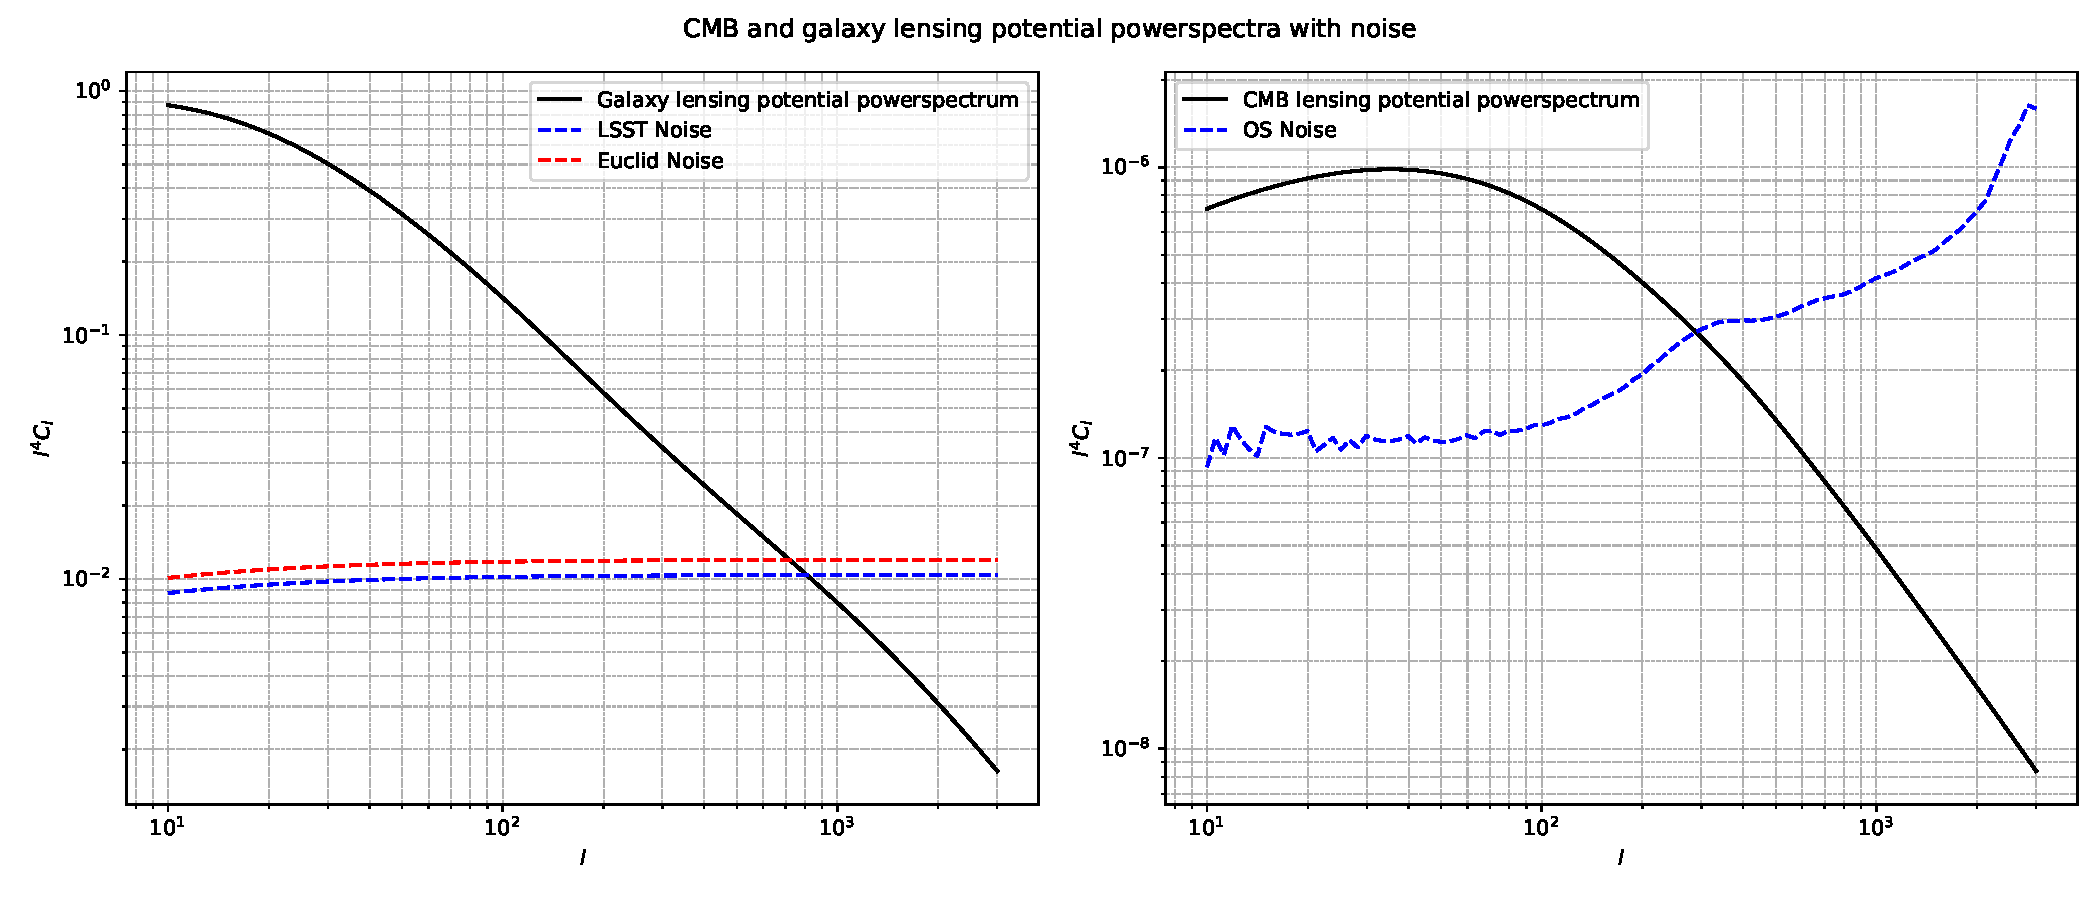
\includegraphics[width=\textwidth]{/Users/jonasfrugte/Desktop/Research_Project/fisher_calc_weak_lensing/code/plots/spectraplusnoise.pdf}
    \caption{CMB (right) and galaxy (left) lensing potential power spectra compared to associated experimental noise. Current (stage 3) noise values are displayed as well as near future (stage 4) noi se values. The CMB lensing experiment does not measure temperature anisotropies, only polarization. CMB noise values are chosen in accordance with \cite{Namikawa_2016}. Shear noise values are chosen to be similar to e.g. Euclid measurements for stage 4 and e.g. KiDS for stage 3.}
    \label{fig:lpsplusnoise}
\end{figure}


% For noise in CMB lensing we consider lensing estimated by an experiment measuring polarization with white noise $\Delta_P$ and beam spread $\sigma$. We then use the quadratic estimator from \cite{Hu_2002} to estimate the resulting noise in the lensing power spectrum.




% For shear measurements, the noise is simpler to model as the primary source is shot noise due to the discrete number of galaxies in each patch of the survey. The mean ellipiticity of the galaxies in a patch is calculated and a deviation from the mean is interpreted as lensing shear. The greater the number of galaxies the more accurately can the mean ellipticity be determined. Choosing the size of the patch is a balancing between signal to noise and resolution. Smaller patches give more uncertain shear measurements while providing better overal resolution for the shear map and thus allowing measurements of shear bi- and powerspectra to higher multipole numbers. The opposite is true for larger patch sizes. The power spectrum of the shear noise is given by
% \begin{equation*}
%     N^{\gamma\gamma}_{l} = \frac{\sigma^2_{rms}}{\bar n_g}
% \end{equation*}
% where $\bar n_g$ is the mean number of galaxies observed per sterradian accross the whole survey \cite{weaklensingnotes2020}.
% and $\sigma^2_\gamma$ is the intrinsic ellipticity dispersion. 
% Experiments such as Euclid and the LSST both have $\sigma_{rms} \approx 0.3$ \cite{euclid1overview} \cite{lsstsciencebook} and 
% $ n_g\approx 30 \text{ arcmin}^{-2}$.

% The noise values are calculated for stage 3 (current) surveys and stage 4 (near future) surveys. We will use the stage 4 noise values for parameter constraints. A comparison of stage 3 noise, stage 4 noise, and lensing signal can be seen in figure \ref{fig:lpsplusnoise}.

The redshift distribution of the observed galaxies is commonly parameterized as \cite{bartelmann2001weak}
\begin{equation*}
    n(z) \propto z^a \exp\sbr{-\br{\frac{z}{z_0}}^b}.
\end{equation*}
We choose the parameter combination $a = 2$, $b = 3/2$ and $z_0 = 0.64$ which is similar to the expected distributions of Euclid, (which will probe primarily in the 0.2 - 2.6 redshift range \cite{euclidprep10})
and the LSST mission (which has $a \approx 2$, $b \approx 1$, and $z_0 \approx 0.3$ from predictions for the obtained data \cite{lsstsciencebookchapter3}).

\section{Results}\label{sec:results}
\subsection{SNR}
Lensing power spectra are well detectable in nearly all cases. 
The signal to noise ratios of the CMB and galaxy lensing bispectra v.s. the maximum multipole moment measured can be found in figure \ref{fig:snrplots}. Shear bispectra can be measured well by both stage 3 and stage 4 experiments, while CMB lensing is only semi detectable by a stage 3 experiment but well detectable by stage 4 experiments.
%It can be seen that the CMB bispectrum signal to noise never exceeds 2 even for $l_{\max} = 2000$, meaning that this signal is not likely to be able to contribute to parameter constraints in future surveys. All other quantities should be well detectable for $l_{\max}\geq 500$.
\begin{figure}
    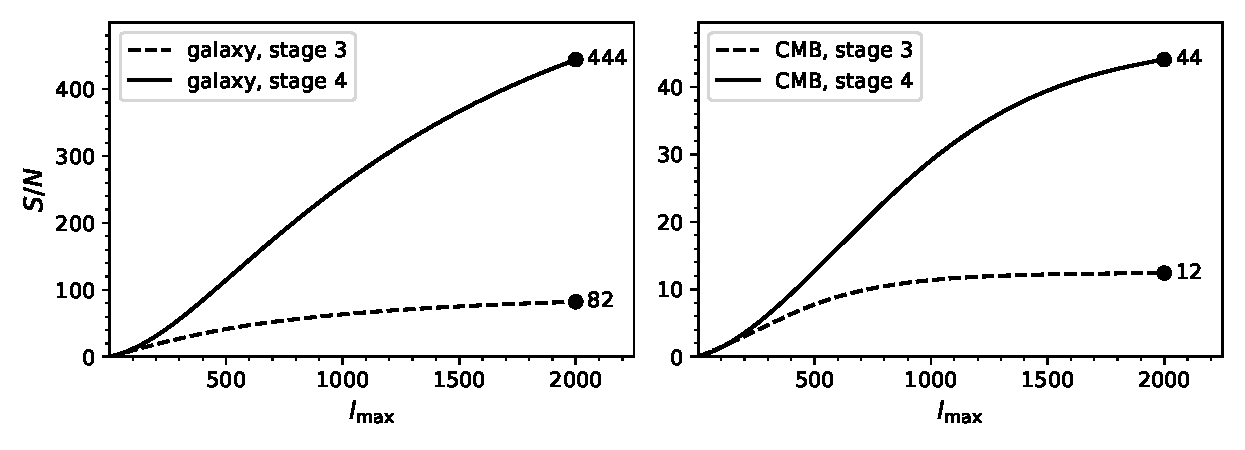
\includegraphics[width=\textwidth]{figures/snrplots.pdf}
    \caption{Signal to noise ratios for galaxy lensing (dashed) and CMB lensing (non-dashes) power- (in red) and bispectra (in blue). The $x$-axis labels the maximum multipole moment measured up to, starting from $l_{\min}=2$.}
    \label{fig:snrplots}
\end{figure}

\subsection{Parameter Constraints}
For the parameter constraints, even when combining all signals, most of the parameters are poorly constrained (with minimum uncertainties much bigger than their fiducial values). The combination that is well constrained is $H_0$ and $\sigma_8$. Alternatively one can also look at $H_0$ and $S_8$, where $S_8$ is defined as 
\begin{equation*}
    S_8 = \sigma_8 \sqrt{\frac{\Omega_c + \Omega_b}{0.3}}
\end{equation*}
and is commonly found to be a particularly well constrained parameter in weak lensing surveys. The results are essentially the same so we will stick with $\sigma_8$. The constraints and covariances are shown in figures \ref{fig:side_by_side} (a) and (b). In particular, you can see in  the off diagonal plot that combining the CMB and galaxy lensing removes approximate degeneracies in $H_0$, $\sigma_8$ space to create a much smaller $1\sigma$ confidence ellipse. When comparing powerspectra to bispectra constraints in figure \ref{fig:S8const} we see a more mild improvement in constraints when combining the different sources of information.
% \begin{figure}[htbp]
%     \centering
%     \begin{subfigure}[t]{0.48\textwidth}
%         \centering
%         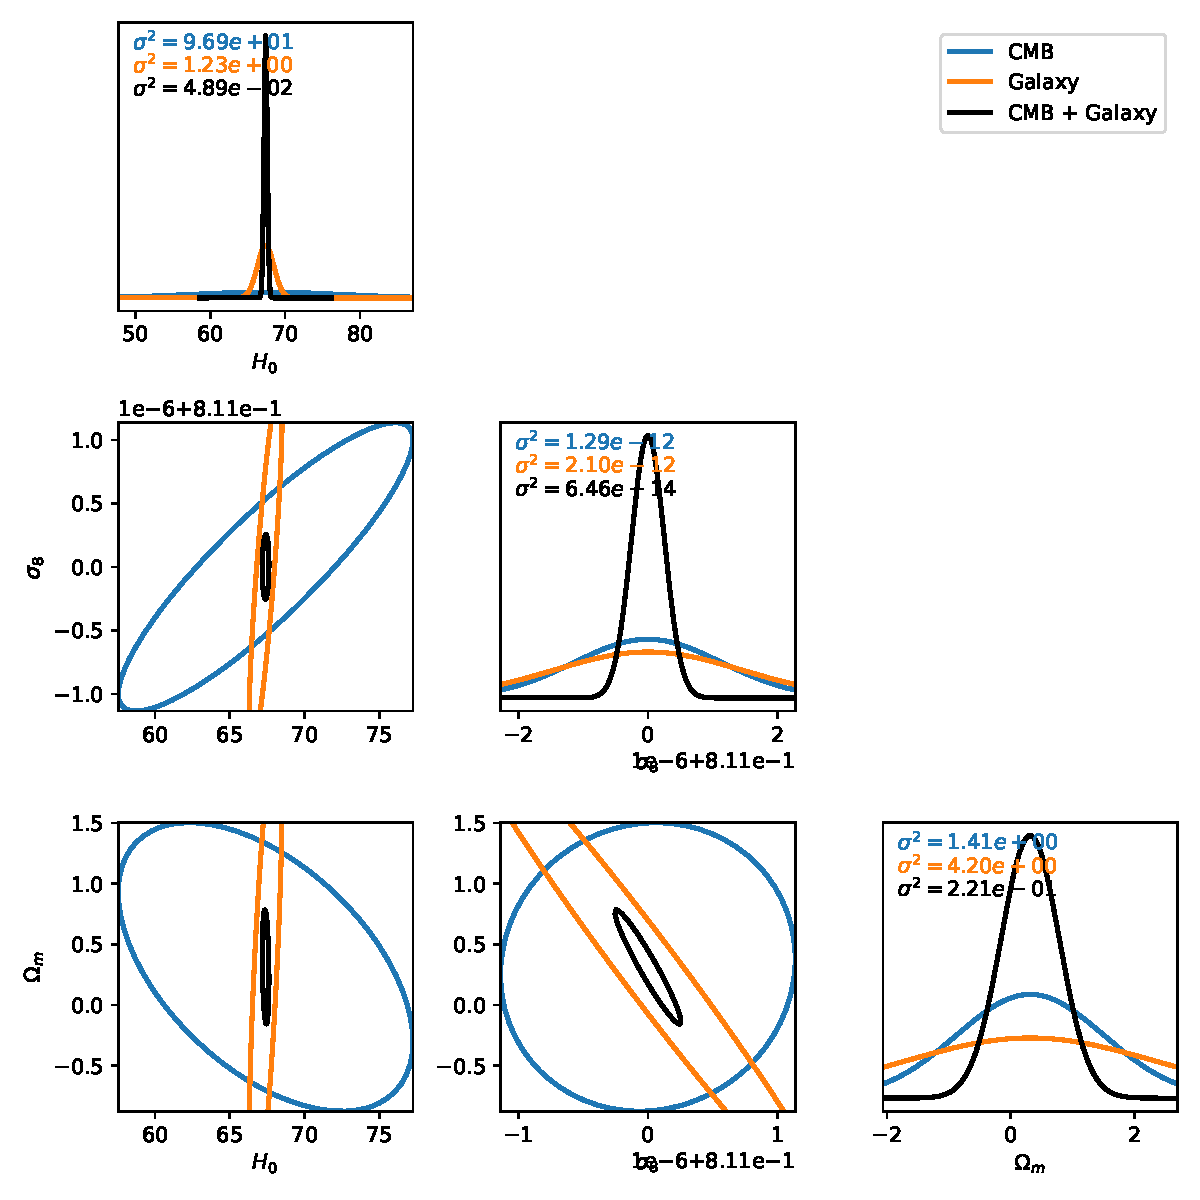
\includegraphics[width=\textwidth]{paramconstraints_sigma8.pdf}
%         
%         \label{fig:sigma8const}
%     \end{subfigure}
%     \hfill
%     \begin{subfigure}[t]{0.48\textwidth}
%         \centering
%         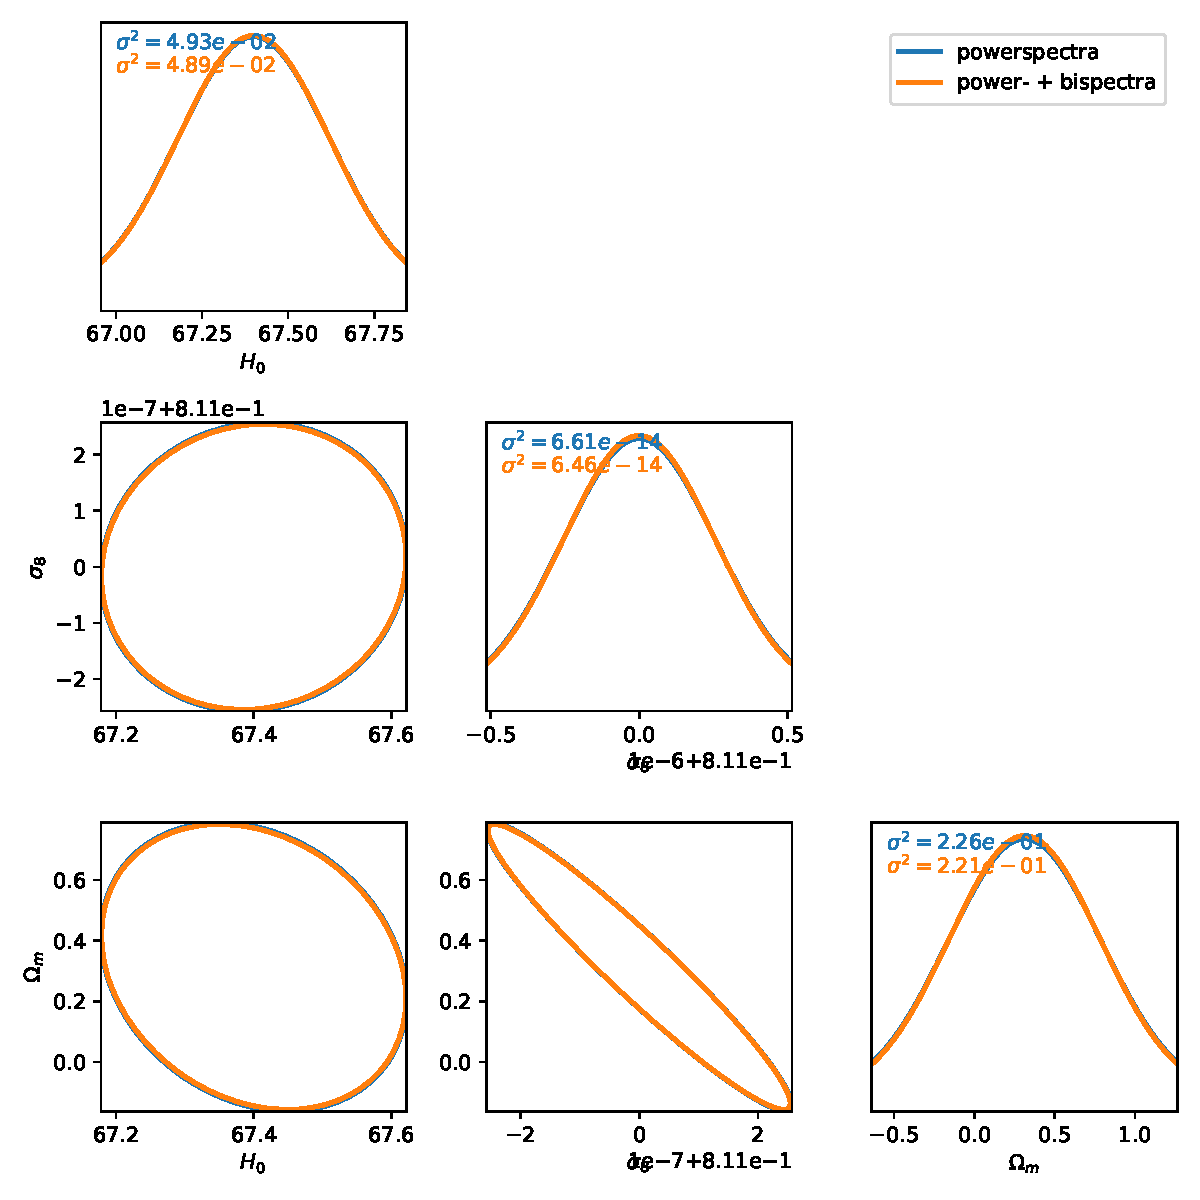
\includegraphics[width=\textwidth]{paramconstraints_sigma8_diffspectra.pdf}
%         \caption{Same as Fig.~\ref{fig:sigma8const}, except comparing constraints from only using power spectra, only bispectra, or both. $S_8$ instead of $\sigma_8$. In all three cases we use CMB $and$ galaxy lensing.}
%         \label{fig:S8const}
%     \end{subfigure}
%     \caption{Side-by-side comparison of parameter constraints.}
%     \label{fig:side_by_side}
% \end{figure}

\begin{figure}
    \centering
    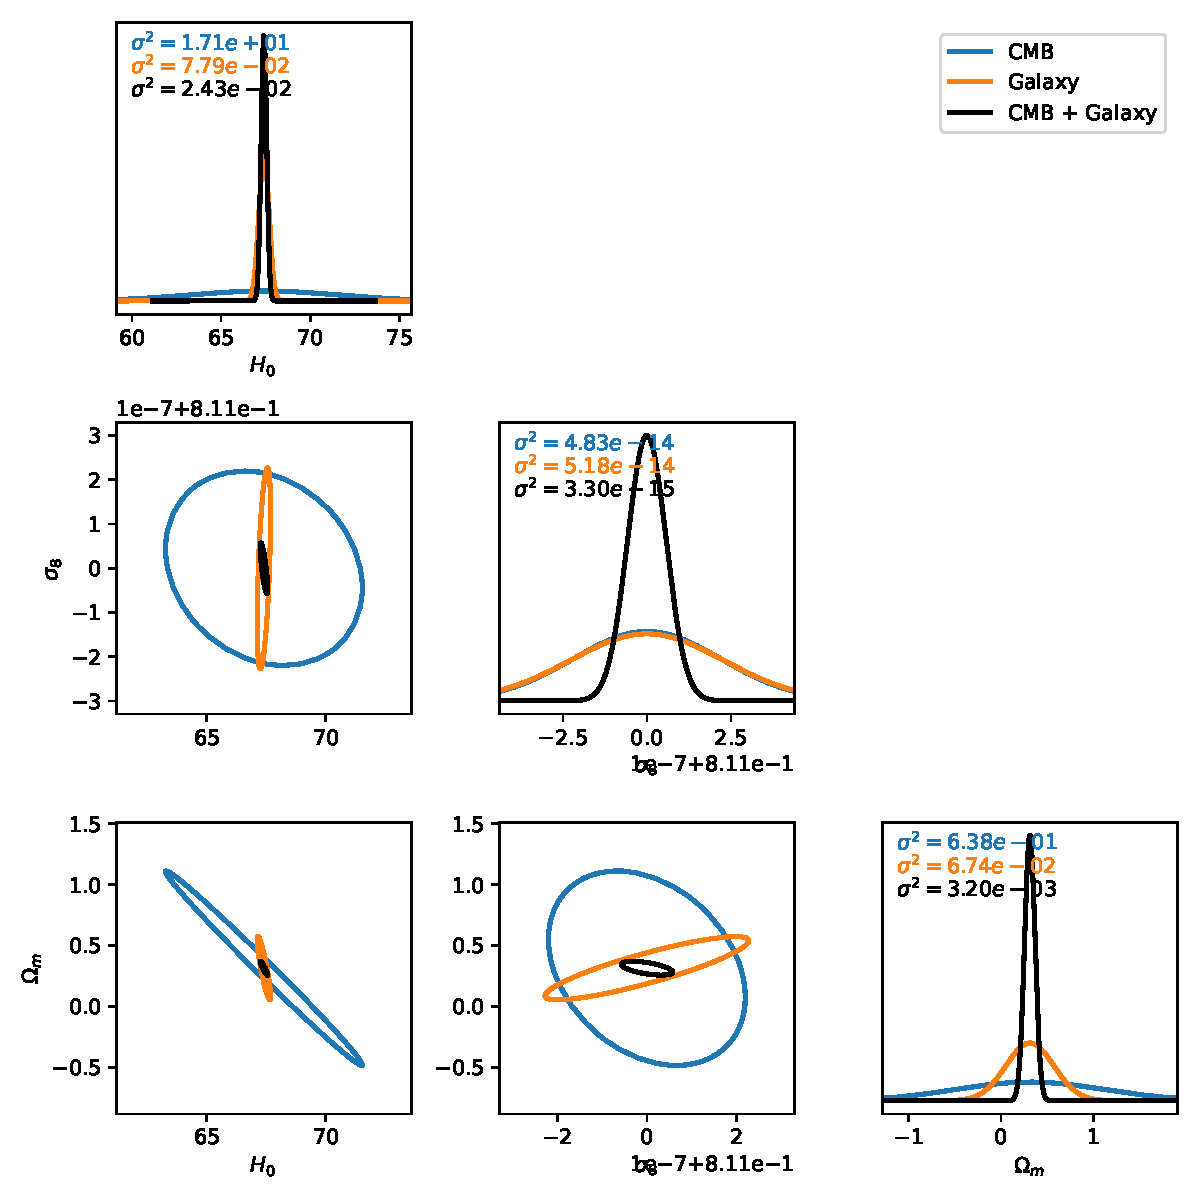
\includegraphics[width=\textwidth]{figures/paramconstraints_difftracers.pdf}
    \caption{Constraints for $H_0$ and $\sigma_8$ for CMB lensing, galaxy lensing, and CMB + galaxy lensing combined. We use the information from both power and bispectra together with $l_{\max}=2000$ in all three cases. The confidence ellipses are for $1\sigma$ certainty.}
    \label{fig:difftracer}
\end{figure}
\begin{figure}
    \centering
    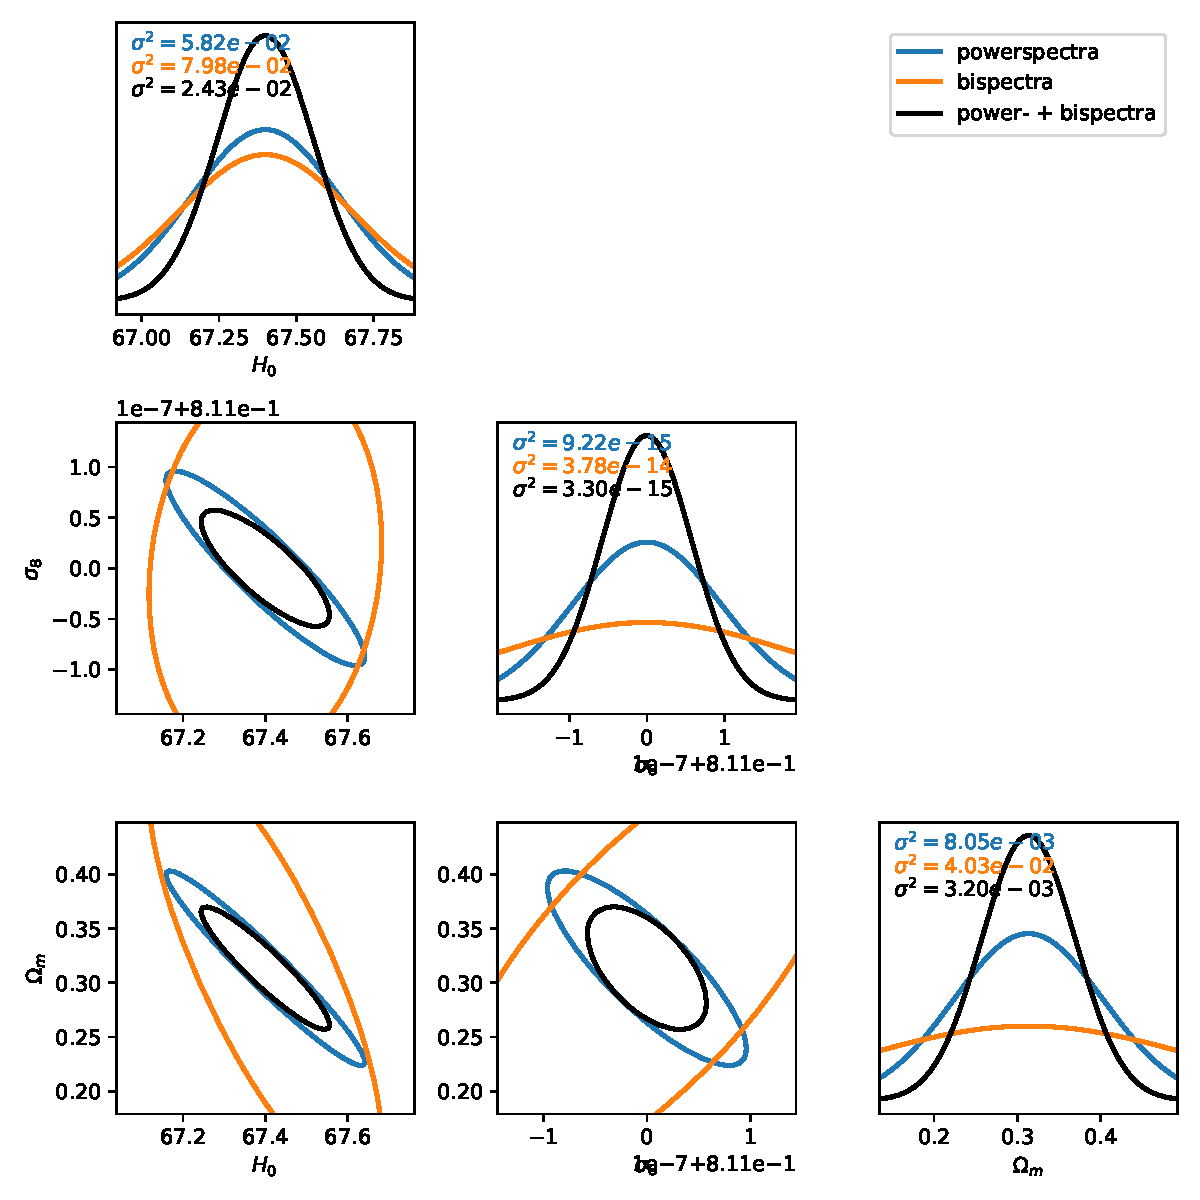
\includegraphics[width=\textwidth]{figures/paramconstraints_diffspectra.pdf}
    \caption{Same as Fig. \ref{fig:difftracer}, except comparing constraints from only using power spectra, only bispectra, or both. In all three cases we use CMB $and$ galaxy lensing.}
    \label{fig:diffspectra}
\end{figure}

\section{Discussion and conclusion}\label{sec:discussion}
% \bibliographystyle{alpha} % Choose your citation style
\printbibliography

\appendix

\section{Weak Lensing}\label{sec:weaklensing}
\subsection{Perturbed Photon Paths}
We work in the conformal newtonian gauge and with natural units. Denoting conformal time and conformal radial distance by $\eta$ and $\chi$, respectively, the perturbed line element in FLRW spacetime is given by
\begin{equation}
    \d s^2 = a^2(\eta)((1 + 2\Psi_N) \d \eta^2 - (1 + 2\Phi_N) \gamma_{ij}\d x^i \d x^j),
\end{equation}
where $\gamma_{ij}$ is the unperturbed line element
\begin{equation}
    \gamma_{ij} = \d x^i \d x^j = \d \chi^2 + f^2_K(\chi)(\d \theta^2 + \sin ^2 \theta \d \phi ^2),
\end{equation}
and $f_K(\chi)$ is the comoving angular diameter distance. We will hereafter only consider a flat universe, so that $f_K(\chi) = \chi$. Weak lensing of a point source can be quantified by looking at the deflection field $\mathbf d (\hat{\mathbf n}) = \mathbf \theta_{\text{obs}} - \mathbf \theta_{\text{true}}$, i.e. the (small) difference between the angle at which we see the object and the angle at which we would see the object had no lensing occured. To first order in $\Psi_N$ and $\Phi_N$, the deflection is given as \cite{dodelson2020modern}
\begin{equation}
    \mathbf d(\hat{\mathbf n}) = -2 \int_0^{\chi_*}\d \chi \frac{\chi_* - \chi}{\chi_*\chi}\nabla_{\hat{\mathbf n}}\Psi(\chi\hat{\mathbf n};\eta_0 - \chi),
\end{equation}
where $\Psi$ is the Weyl Potential, $\Psi := (\Psi_N - \Phi_N)/2$, and $\chi_*$ is the conformal distance to the source. $\nabla_{\hat{\mathbf n}}$ is the derivative along the axes orthogonal to the line of sight. The above equation can be written in terms of the lensing potential, $\psi$, as $\mathbf d (\hat{\mathbf n}) = \nabla_{\hat{\mathbf n}} \psi(\hat{\mathbf n})$, with
\begin{equation}
    \psi(\hat {\mathbf n}) := -2 \int_0^{\chi_*}\d \chi \frac{\chi_* - \chi}{\chi_*\chi}\Psi(\chi\hat{\mathbf n};\eta_0 - \chi).
\end{equation}

If the source is instead distributed over radial distance according to some distribution function $p(\chi)$, with $p(\chi)$ normalized to integrate to 1, the $(\chi_* - \chi)/(\chi_*\chi)$ factor is changed as
\begin{equation*}
    \frac{\chi_*-\chi}{\chi_*\chi} \rightarrow W(\chi) := \int_\chi^{\infty}\d\chi' p(\chi')\frac{\chi'-\chi}{\chi'\chi}.
\end{equation*}
$W(\chi)$ is then called the window function. In the most general case, the lensing potential is thus given by
\begin{equation}
    \psi(\hat {\mathbf n}) := -2 \int_0^{\infty}\d \chi W(\chi)\Psi(\chi\hat{\mathbf n};\eta_0 - \chi).
\end{equation}
The integration limit is sometimes also taken to be the surface of last scattering, as any window function vanishes after that distance. In the case of CMB lensing we can take $p(\chi')=\delta(\chi'-\chi_*)$, in which case the window function reduces to $H(\chi_* - \chi)(\chi_*-\chi)/(\chi_*\chi)$, with $H(\chi)$ the Heaviside step function.

% From here of on work in first order in the scalar potentials $\Phi_N$ and $\Psi_N$. For lensing we consider null-geodesics so $\d s^2 = 0$ and we can rewrite the perturbed line element as
% \begin{equation}
%     \d \hat s^2 = (1 + 4\Psi)\d\eta^2 - \gamma_{ij} \d x^i \d x^j
% \end{equation}
% with $\Psi$ the \textbf{Weyl Potential} given by $\Psi := (\Psi_N - \Phi_N)/2$. A null geodesic $x^\mu(\hat\lambda)$ in terms of its affine parameter ($\hat \lambda$) satisfies the geodesic equation
% \begin{equation}
%     \frac{\d^2 x^\mu}{\d \hat\lambda^2} + \Gamma^\mu_{\nu\rho} \frac{\d x^\nu}{\d \hat\lambda}\frac{\d x^\rho}{\d\hat\lambda} = 0,
% \end{equation}
% with $\hat g_{\mu\nu}(\d x^\mu/\d \hat\lambda)(\d x^\nu / \d \hat \lambda) = 0$. 

% In the unperturbed there are incoming radial solutions of the form $\chi = \eta_0 - \eta$. We can express $\hat\lambda$ in terms of $\eta$ using The 0-component of the geodesic equation,
% \begin{equation}
%     \frac{\d^2\eta}{\d\hat\lambda^2} + 2(\frac{\d\eta}{\d\hat\lambda})^2\frac{\d\Psi}{\d\eta}+2\frac{\d\eta}{\d\hat\lambda}\frac{\d x^i}{\d\hat\lambda}\frac{\partial\Psi}{\partial x^i} = 0,
% \end{equation}
% where the derivative $\d\Psi/\d\eta = \partial_\eta\Psi+(\d x^i/\d\eta)\partial_i\Psi$ is along the perturbed ray. This allows us to rewrite the other (spatial) geodesic equations as
% \begin{equation}
%     \frac{\d^2x^i}{\d\eta^2} - 2\frac{\d x^i}{\d\eta}(\frac{\d\Psi}{\d\eta} + \frac{\d x^j}{\d\eta}\frac{\partial\Psi}{\partial x^j})+2\gamma^{ij}\frac{\partial\Psi}{\partial x^j}+\bar\Gamma^i_{jk}\frac{\d x^j}{\d\eta}\frac{\d x^k}{\d \eta} = 0,
% \end{equation}
% where $\bar\Gamma^i_{jk}$ are the connection coefficients of the unperturbed three geometry $\gamma_{ij}$. Without loss of generality we consider an observer located at the origin of the spatial coordinates, meaning we are interested in rays that end at $x^i = 0$. In that case $\d \chi/\d \eta = -1 + O(\Psi)$, $\d \theta/\d\eta = O(\Psi)$ and $\d \phi/\d\eta = O(\Psi)$ (with $\theta$ and $\phi$ angular spatial coordinates). For the case of such rays we can evaluate the connection coefficients and rewrite the spatial geodesic equations as
% \begin{gather}
%     \frac{\partial^2\chi}{\d\eta^2}+2\frac{\d\Psi}{\d\eta}=0,\\
%     \frac{\d^2\theta}{\d\eta^2}-2\frac{\d\ln f_K(\chi)}{\d\chi}\frac{\d\theta}{\d\eta}+\frac{2}{f^2_K(\chi)}\frac{\partial\Psi}{\partial\theta}=0,\\
%     \frac{\d^2\phi}{\d\eta^2} - 2\frac{\d \ln f_K(\chi)}{\d\chi}\frac{\d\phi}{\d\eta}+\frac{2}{f^2_K(\chi)}\frac{1}{\sin^2(\theta)}\frac{\partial\Psi}{\partial\phi}=0.
% \end{gather}
% Integrating twice and using the null condition we can rewrite the the first equation as
% \begin{equation}
%     \chi = \eta_0 - \eta - 2\int_{\eta_0}^\eta\Psi\d\eta',
% \end{equation}
% where the integral is along the ray. Since we are working at first order in $\Psi$ we can evaluate the integral along the unperturbed path, this is known as the \textbf{Born approximation}.\textit{Next follows a short discussion of why perturbations in observation time can be ignored, include?} Doing the same for the other two equations gives
% % TODO: make n a proper vector (bold)
% \begin{gather}
%     \theta(\eta_0 - \chi_*)=\theta_0 - \int_0^{\chi_*}\d\chi\frac{f_K(\chi_* - \chi)}{f_K(\chi_*)f_K(\chi)}2\frac{\partial}{\partial \theta}\Psi(\chi\hat n, \eta_0 - \chi),\\
%     \phi(\eta_0 - \chi_*)=\theta_0 - \int_0^{\chi_*}\d\chi\frac{f_K(\chi_* - \chi)}{f_K(\chi_*)f_K(\chi)}\frac{2}{\sin^2\theta}\frac{\partial}{\partial \phi}\Psi(\chi\hat n, \eta_0 - \chi),
% \end{gather}
% where $\theta_0$ and $\phi_0$ label the line of sight $\hat n$. The displacement vector $\mathbf{\alpha}$ indicates the infinitesimal displacement of the lensed rays from their unpetrubed observed angles and is related to $\theta$ and $\phi$ through
% $$
% \alpha_\theta = \theta - \theta_0, \quad \alpha_\phi = \sin^2\theta(\phi - \phi_0).
% $$
% An object 
% \begin{equation}
%     \mathbf \alpha = -2 \int_0^{\chi_*}\d \chi \frac{f_K(\chi_* - \chi)}{f_K(\chi_*)f_K(\chi)}\nabla_{\hat{\mathbf n}}\Psi(\chi\hat{\mathbf n};\eta_0 - \chi).
% \end{equation}
% When working in the weak field limit (i.e. small spacetime curvature) the $00$ component of Einsteins equations give us a poisson equation \cite{dodelson2020modern},
% \begin{equation}
%     -\nabla^2\Psi(\textbf{x}, \eta) =  4\pi G a(\eta)^2\delta\rho(\mathbf x, \eta)
% \end{equation}
% where $K$ is $0$, $1$, or $-1$ depending on the curvature of the universe, $\Delta = \partial_x^2 + \partial_y^2 + \partial_z^2$ is the 3 dimensional laplace operator, $\delta\bar\rho$ is the comoving total energy perturbation (evaluated in the rest-frame of the total energy). %TODO: proper definition for anisotropic stress and explain why we can ignore it

\subsection{Convergence and Shear}
The magnification matrix is defined as
\begin{equation}
    A_{ij} := \delta_{ij} + \frac{\partial}{\partial n_j}d_i(\hat{\mathbf n}).
\end{equation}
This matrix can be decomposed in the following form, which immediately gives us definitions for the \textbf{convergence}, $\kappa$, \textbf{shear}, $\gamma_1$ and $\gamma_2$, and \textbf{rotation}, $\omega$:
\begin{equation}
    A_{ij}(\hat{\mathbf n}) = \begin{pmatrix}
        1 - \kappa - \gamma_1 & -\gamma_2 + \omega \\
        -\gamma_2 - \omega & 1 - \kappa + \gamma_1
    \end{pmatrix}.
\end{equation}
At 1st order $A$ is a symetric matrix by definition and $\omega$ vanishes, we will ignore it from here on out. Intuitively, $A$ tells you how a small patch in the sky transforms due to lensing. If we change the unlensed direction of a light source by $\delta\hat{\mathbf n}$, then the corresponding change in direction in the lensed image can be calculated as
\begin{equation}
\hat{\mathbf{n}} + \delta \hat{\mathbf{n}} \rightarrow \hat{\mathbf{n}} + \delta \hat{\mathbf{n}} + \mathbf d (\hat{\mathbf{n}} + \delta \hat{\mathbf{n}}) = \hat{\mathbf{n}} + \mathbf d (\hat{\mathbf n}) + \delta \hat{\mathbf n} + A_{ij}(\delta \hat{\mathbf{n}})_j.
\end{equation}
For an image on the sky, $A_{ij}$ thus introduces distortion. Note that $|A_{ij}| = (1 - \kappa)^2 + \omega^2 - |\gamma|^2 = 1 - 2\kappa + O(\kappa^2, \gamma^2, \omega^2)$. We can thus interpret $\kappa$ as telling us about the overal magnification of the source. The $\gamma_i$ represent the area preserving distortion, i.e. stretching and squeezing in a specific direction.

We can relate $\kappa$ and $\gamma$ directly to the lensing potential as
% TODO: should these subscripts be theta and phi?
\begin{equation}
    \kappa = \frac{1}{2}\nabla^2\psi, \quad \gamma_1 = \frac{1}{2}(\partial_{n_1}^2 - \partial_{n_2}^2)\psi, \quad \gamma_2 = \partial_{n_1}\partial_{n_2} \psi.
\end{equation}

\section{Weak Lensing Statistics}\label{sec:weaklensstats}
\subsection{Lensing Potential Powerspectrum}
The lensing potential can be decomposed into spherical harmonics as
\begin{equation}
    \psi(\hat{\mathbf n}) = \sum_{lm} \psi_{lm}Y_{lm}(\hat{\mathbf n}).
\end{equation}
On the other hand, consider the decomposition of $\Psi$ in Fourier modes with the Fourier convention $\Psi(\mathbf x, \eta)=\int\frac{\d^3 \mathbf k}{(2\pi)^{3}}\Psi(\mathbf k, \eta)e^{i\mathbf k \cdot\mathbf x}$,
\begin{equation}
    \psi(\hat{\mathbf n}) = -2 \int_0^{\chi_*}\d \chi W(\chi) \int\frac{\d^3 \mathbf k}{(2\pi)^{3}}\Psi(\mathbf k, \eta_0 - \chi)e^{i\mathbf k \cdot\hat{\mathbf n}\chi}.
\end{equation}
We can than relate the multipole modes of $\psi$ to the fourier modes of $\Psi$ through % TODO: check sign convention here
\begin{gather}
    \psi_{lm} = \langle Y_l^m | \psi \rangle = \int\d^2\hat{\mathbf n} Y_l^m(\hat{\mathbf n})^* \psi(\hat{\mathbf n})\\ 
    = -2\int\d^2\hat{\mathbf n} Y_l^m(\hat{\mathbf n})^* \int_0^{\chi_*}\d \chi W(\chi) \int\frac{\d^3 \mathbf k}{(2\pi)^{3}}\Psi(\mathbf k, \eta_0 - \chi)e^{i\mathbf k \cdot\hat{\mathbf n}\chi}
\end{gather}
Now define the power spectrum as
\begin{equation}
    \langle \Psi(\mathbf k, \eta)\Psi(\mathbf k',\eta')\rangle = \frac{2\pi^2}{k^3}P_\Psi(k, \eta, \eta')\delta(\mathbf k + \mathbf k'),
\end{equation}
with $\eta$ denoting the conformal time. This gives 
%TODO: define the window function
\begin{equation}
    \langle \psi(\hat{\mathbf n})\psi(\hat{\mathbf n}') \rangle = 4\int_0^{\chi_*}\d \chi\int_0^{\chi_*}\d \chi' W(\chi)W(\chi')\int \frac{\d^3\mathbf k}{(2\pi)^6}\frac{2\pi^2}{k^3}P_\psi(k,\eta_0 - \chi, \eta_0-\chi')e^{i\mathbf k\cdot\hat {\mathbf n}\chi}e^{-i\mathbf k\cdot\hat {\mathbf n}'\chi'},
\end{equation}
where we used that $\eta = \eta_0 - \chi$ along the unperturbed photon path (this is known as the Born approximation), with $\eta_0$ the time at which the light ray hits earth. 
We can use the result
\begin{equation}
    e^{i\mathbf k \cdot \hat {\mathbf n}\chi}=4\pi\sum_{lm}i^lj_l(k\chi )Y_l^m(\hat{\mathbf n})^*Y_l^m(\hat{\mathbf k}) = 4\pi\sum_{lm}i^lj_l(k\chi )Y_l^m(\hat{\mathbf n})Y_l^m(\hat{\mathbf k})^*, \label{eq:complexexp}
\end{equation}
where $j_l$ is the spherical Bessel function, to rewrite the above equation. Using both versions of the identity above, we immediately get a factor $Y_l^m(\hat{\mathbf k})Y_{l'}^{m'}(\hat{\mathbf k})^*$ in our integral. We can factor the differential element of $\d^3\mathbf k$ into a radial and angular part as $k^2\d k\d^2\Omega_k$, with $\Omega_k$ the solid angle, to apply the orthonormality condition of the spherical harmonics. Note that we take the same sequence of steps a number of times in other parts of the derivations of the lensing spectra. We thus obtain
\begin{gather}
    \langle \psi(\hat{\mathbf n})\psi(\hat{\mathbf n}') \rangle = 4(4\pi)^2\sum_{ll'mm'}i^{l-l'}\int_0^{\chi_*}\d \chi\int_0^{\chi_*}\d \chi' W(\chi)W(\chi')\\\times\int \frac{k^2\d k}{(2\pi)^6}\frac{2\pi^2}{k^3}j_l(k\chi)j_{l'}(k\chi')P_\psi(k,\eta_0 - \chi, \eta_0-\chi')Y_{lm}(\hat{\mathbf n})Y_{l'm'}(\hat{\mathbf n}')^*\delta_{ll'}\delta_{mm'}. \label{eq:lenspotcorrexpanded}
\end{gather}
The angular power spectrum is defined similarly to the power spectrum, i.e.
\begin{equation}
    \langle \psi_{lm}\psi_{l'm'}^* \rangle = \delta_{ll'}\delta_{mm'}C_l^\psi.
\end{equation}
Note that the correlation is independent of $m$ and $m'$. %TODO: explain how this relates to statistical isotropy
We can thus read from equation \ref{eq:lenspotcorrexpanded} that
\begin{gather}
    C_l^\psi = 4(4\pi)^2\int_0^{\chi_*}\d \chi\int_0^{\chi_*}\d \chi' W(\chi)W(\chi')\int \frac{k^2\d k}{(2\pi)^6}\frac{2\pi^2}{k^3}j_l(k\chi)j_{l}(k\chi')P_\psi(k,\eta_0 - \chi, \eta_0-\chi'),
\end{gather}
which can be simplified to
\begin{gather}
    C_l^\psi = \frac{2}{\pi^2}\int_0^{\chi_*}\d \chi\int_0^{\chi_*}\d \chi' W(\chi)W(\chi')\int k^2\d kj_l(k\chi)j_{l}(k\chi')\frac{P_\psi(k,\eta_0 - \chi, \eta_0-\chi')}{k^3}.
\end{gather}

To further evaluate the integral we will make the Limber approximation. The Bessel functions peak sharply at $l=x$\footnote{Some sources use $x\approx l+1/2$ instead, which is slightly more accurate for larger scales (low $l$) and slightly less accurate for smaller scales.}, with the peak being increasingly sharp for higher $l$. Similarly to $\delta(x-x_0)f(x)=\delta(x-x_0)f(x_0)$, we thus take $j_l(k\chi)f(k)\approx j_l(k\chi)f(l/\chi)$. The Bessel functions satisfy an orthogonality condition,
\begin{equation}
    \int k^2\d k j_l(k\chi)j_l(k\chi') = \frac{\pi}{2\chi^2}\delta(\chi-\chi').
\end{equation}
In combination with the Limber approximation we thus find
\begin{equation}
    \int k^2\d k j_l(k\chi)j_l(k\chi')f(k) \approx \frac{\pi}{2\chi^2}\delta(\chi-\chi')f(l/\chi).
\end{equation}
%TODO: how high? quantify limber approx, perhaps using convergence x LSS paper
It allows us to write the Limber-approximate angular spectrum as
\begin{gather}
    C^\psi(l) = \frac{2}{\pi^2}\int_0^{\chi_*}\d \chi\int_0^{\chi_*}\d \chi' W(\chi)W(\chi') \frac{\pi}{2\chi^2}\delta(\chi-\chi')\frac{\chi^3}{l^3}P_\psi(l/\chi,\eta_0 - \chi, \eta_0-\chi')\\
    = \frac{1}{l^3\pi}\int_0^{\chi_*}\chi\d \chi W(\chi)^2 P_\psi(l/\chi,\eta_0 - \chi, \eta_0-\chi). \label{eq:lpsintermsofpsi}
\end{gather}
% The power spectrum of the potential can be related to the power spectrum of the matter density using the Poisson equation %TODO: create ref
% For a flat universe in atter or dark energy domination we thus find the relation
% \begin{equation}
%     P_\Psi(k;\eta, \eta)=\frac{9\omega_m^2(\eta)H^4(\eta)}{8\pi^2} \frac{P_m(k, \eta)}{k},
% \end{equation}
% where we use the shorthand $P_m(k, \eta):=P_m(k,\eta,\eta)$. The lensing power spectrum is thus finally given in terms of the matter power spectrum as
% \begin{equation}
%     C_l^\psi=\underbrace{9\omega_m^2(\eta)H^4(\eta)}_{:=C(\eta)}\frac{1}{l^4}\int_0^{\chi_*}\d\chi\chi^2 W(\chi)^2P_m(l/\chi, \eta_0-\chi).
% \end{equation}
% We will henceforth denote the $\eta$ dependent factor outside of the integral as $C(\eta)$.
\subsection{Lensing potential bispectrum}
The derivation of the bispectrum proceeds similarly to that of the power spectrum. We aim to compute the bispectrum of the lensing potential fields of 3 (possibly distinct sources), $\psi_1$, $\psi_2$, $\psi_3$. 
\begin{gather*}
    \langle (\psi_1)_{l_1m_1}(\psi_2)_{l_2m_2}(\psi_3)_{l_3m_3} \rangle = 
    \prod_i\br{-2\int\d^2\hat{\mathbf n_i}(Y^{m_i}_{l_i}(\hat{\mathbf n_i}))^*\int_0^{\chi_*}\d\chi_i W_i(\chi_i)\int\frac{\d^3\mathbf k_i}{(2\pi)^{3}}e^{i\mathbf k_i \cdot\hat{\mathbf n_i}\chi_i}} \\
    \times \langle \prod_i\Psi(\mathbf k_i, \eta_0 - \chi_i) \rangle.
\end{gather*}
Defining the bispectrum of the graviational potential as
\begin{equation*}
    \langle \prod_{i=1,2,3}\Psi(\mathbf k_i, \eta_0 - \chi_i) \rangle = (2\pi)^3\delta(\mathbf k_1 + \mathbf k_2 + \mathbf k_3)B^\Psi(\{k_i\}, \{\eta_0-\chi_i\}),
\end{equation*}
we rewrite the lensing potential bispecrum as
\begin{gather*}
    \langle (\psi_1)_{l_1m_1}(\psi_2)_{l_2m_2}(\psi_3)_{l_3m_3} \rangle = 
    \prod_i\br{-2\int\d^2\hat{\mathbf n_i}(Y^{m_i}_{l_i}(\hat{\mathbf n_i}))^*\int_0^{\chi_*}\d\chi_i W_i(\chi_i)\int\frac{\d^3\mathbf k_i}{(2\pi)^{3}}e^{i\mathbf k_i \cdot\hat{\mathbf n_i}\chi_i}}\\ \times (2\pi)^3\delta(\mathbf k_1 + \mathbf k_2 + \mathbf k_3)B^\Psi(\{k_i\}, \{\eta_0-\chi_i\}).
\end{gather*}
Now using equation \ref{eq:complexexp} to rewrite the complex exponential:
\begin{gather*}
    \langle (\psi_1)_{l_1m_1}(\psi_2)_{l_2m_2}(\psi_3)_{l_3m_3} \rangle \\ = 
    \prod_i\br{-2\int\d^2\hat{\mathbf n_i}(Y^{m_i}_{l_i}(\hat{\mathbf n_i}))^*\int_0^{\chi_*}\d\chi_i W_i(\chi_i)\int\frac{\d^3\mathbf k_i}{(2\pi)^{3}}4\pi\sum_{lm}i^{l}j_{l}(k_i\chi_i)Y_{l}^{m}(\hat{\mathbf n_i})Y_{l}^{m}(\hat{\mathbf k_i})^*}\\
    \times (2\pi)^3\delta(\mathbf k_1 + \mathbf k_2 + \mathbf k_3)B^\Psi(\{k_i\}, \{\eta_0-\chi_i\}) \\
    = \sbr{\prod_i\br{-2\int_0^{\chi_*}\d\chi_i W_i(\chi_i)\int\frac{\d^3\mathbf k_i}{(2\pi)^{3}}4\pi i^{l_i}j_{l_i}(k_i\chi_i)Y_{l_i}^{m_i}(\hat{\mathbf k_i})^*}} (2\pi)^3\delta(\mathbf k_1 + \mathbf k_2 + \mathbf k_3)B^\Psi(\{k_i\}, \{\eta_0-\chi_i\}).
\end{gather*}
We can write the 3D dirac delta function in terms of spherical harmonics as
\begin{equation*}
    \delta(\mathbf k_1 + \mathbf k_2 + \mathbf k_3) = 8\int\d^3\mathbf x\prod_{i=1,2,3}\br{ \sum_{l_jm_j} i^{l_j}j_{l_j}(k_ix)Y_{l_j}^{m_j}(\hat{\mathbf k_i}) Y_{l_j}^{m_j}(\hat{\mathbf x})^* }.
\end{equation*}
This results in
\begin{gather*}
    \langle (\psi_1)_{l_1m_1}(\psi_2)_{l_2m_2}(\psi_3)_{l_3m_3} \rangle= \prod_i\br{-2\int_0^{\chi_*}\d\chi_i W_i(\chi_i)\int\frac{\d^3\mathbf k_i}{(2\pi)^{3}}4\pi i^{l_i}j_{l_i}(k_i\chi_i)Y_{l_i}^{m_i}(\hat{\mathbf k_i})^*} \\
    \times (2\pi)^38\int\d^3\mathbf x\prod_{i}\br{ \sum_{lm} i^{l}j_{l}(k_ix)Y_{l}^{m}(\hat{\mathbf k_i}) Y_{l}^{m}(\hat{\mathbf x})^* }B^\Psi(\{k_i\}, \{\eta_0-\chi_i\})\\
    = (2\pi)^38\int\d^3\mathbf x\prod_i\br{-2\int_0^{\chi_*}\d\chi_i W_i(\chi_i)\int\frac{k_i^2\d k_i}{(2\pi)^{3}}4\pi (-1)^{l_i}j_{l_i}(k_i\chi_i)j_{l_i}(k_ix) Y_{l_i}^{m_i}(\hat{\mathbf x})^*} B^\Psi(\{k_i\}, \{\eta_0-\chi_i\})
\end{gather*}
The angular part of the $\mathbf x$ integral can be evaluated using the identity
\begin{gather*}
    \int \mathrm{d}\Omega_{\hat{n}} \, Y_{l_1 m_1}^*(\hat{x}) Y_{l_2 m_2}^*(\hat{n}) Y_{l_3 m_3}^*(\hat{n}) = (-1)^{m_1 + m_2 + m_3} 
    \int \mathrm{d}\Omega_{\hat{n}} \, Y_{l_1 -m_1}(\hat{n}) Y_{l_2 -m_2}(\hat{n})Y_{l_3 -m_3}(\hat{n}) \\
    = (-1)^{m_1 + m_2 + m_3} 
    \sqrt{\frac{(2l_1 + 1)(2l_2 + 1)(2l_3 + 1)}{4\pi}} \begin{pmatrix} l_1 & l_2 & l_3 \\ 0 & 0 & 0 \end{pmatrix}
    \begin{pmatrix} l_1 & l_2 & l_3 \\ -m_1 & -m_2 & -m_3 \end{pmatrix} \equiv A_{\mathbf{l}}^{\mathbf{m}},
\end{gather*}
giving
\begin{gather*}
    \langle (\psi_1)_{l_1m_1}(\psi_2)_{l_2m_2}(\psi_3)_{l_3m_3} \rangle 
    = (2\pi)^3 8 A_{\mathbf l}^{\mathbf m}\int x^2\d x\prod_i\br{-2\int_0^{\chi_*}\d\chi_i W_i(\chi_i)\int\frac{k_i^2\d k_i}{(2\pi)^{3}}4\pi (-1)^{l_i}j_{l_i}(k_i\chi_i)j_{l_i}(k_ix)} \\ \times B^\Psi(\{k_i\}, \{\eta_0-\chi_i\}).
\end{gather*}
Now applying the Limber approximation again:
\begin{gather*}
    \langle (\psi_1)_{l_1m_1}(\psi_2)_{l_2m_2}(\psi_3)_{l_3m_3} \rangle 
    = (2\pi)^3 8 A_{\mathbf l}^{\mathbf m}\int x^2\d x\prod_i\br{-2\int_0^{\chi_*}\d\chi_i W_i(\chi_i)\frac{1}{(2\pi)^{3}}\frac{\pi}{2\chi_i^2}\delta(x-\chi_i)4\pi (-1)^{l_i}} \\ \times B^\Psi(\{l_i/\chi_i\}, \{\eta_0-\chi_i\}) \\
    = (2\pi)^3 8 A_{\mathbf l}^{\mathbf m}\int \chi^2\d \chi\prod_i\br{-2 W_i(\chi)\frac{1}{(2\pi)^{3}}\frac{\pi}{2\chi^2}4\pi (-1)^{l_i}} B^\Psi(\{l_i/\chi\}, \eta_0-\chi).
\end{gather*}
Finally, we aim to rewrite the above in terms of the angular bispectrum of the lensing potential. 

The definition for the bispectrum of any set of randomly distributed spherical harmonic components $X^k_{lm}$ is \cite{Hu2000}
\begin{equation*}
    \langle (X_1)_{l_1m_1}(X_2)_{l_2m_2}(X_3)_{x_3m_3} \rangle = \begin{pmatrix}
        l_1 & l_2 & l_3 \\ m_1 & m_2 & m_3
    \end{pmatrix}
    B_{l_1l_2l_3}^{X_1X_2X_3}.
\end{equation*}
Note the independence on $m_i$, this necesarilly follows from statistical isotropy. % TODO: add a short explanation here
If $m_1+m_2+m_3\neq 0$, the associated Wigner-3j symbol vanishes and the bispectrum is set to zero.
Also note that in this definition we have immediately generalized to include cross correlation between different fields $X_1$, $X_2$, $X_3$. This is relevant when we look at cross correlations between CMB and galaxy lensing.
6758
Using the above definition and the symmetry property
\begin{equation*}
    \begin{pmatrix}
        l_1 & l_2 & l_3\\
        -m_1 & -m_2 & -m_3
      \end{pmatrix}
      =
      (-1)^{l_1+l_2+l_3}
      \begin{pmatrix}
        l_1 & l_2 & l_3\\
        m_1 & m_2 & m_3
      \end{pmatrix},
\end{equation*}
we find
\begin{gather*}
    B^{\psi_1\psi_2\psi_3}_{l_1l_2l_3}
    = (-1)^{l_1+l_2+l_3}
    \sqrt{\frac{(2l_1 + 1)(2l_2 + 1)(2l_3 + 1)}{4\pi}} \begin{pmatrix} l_1 & l_2 & l_3 \\ 0 & 0 & 0 \end{pmatrix}
    (2\pi)^3 8 \\
    \times \int \chi^2\d \chi\prod_i\br{-2 W_i(\chi, \chi_*)\frac{1}{(2\pi)^{3}}\frac{\pi}{2\chi^2}4\pi (-1)^{l_i}} B^\Psi(\{l_i/\chi\}, \{\eta_0-\chi\}),
\end{gather*}
where we were able to drop the $(-1)^{m_1+m_2+m_3}$ factor due to the bispecrum vanishing if that sum doesn't equal $0$, as mentioned earlier. When all $m_i$ equal zero, the Wigner 3j-symbol gains a number of useful properties % TODO: discuss all of them
In particular, it vanishes if $l_1+l_2+l_3$ is odd, meaning we can drop the $(-1)^{l_1+l_2+l_3}$ factor. Additionally cancelling common factors then gives
\begin{align}
    B^{\psi_1\psi_2\psi_3}_{l_1l_2l_3}
    =
    -\sqrt{\frac{(2l_1 + 1)(2l_2 + 1)(2l_3 + 1)}{4\pi}} \begin{pmatrix} l_1 & l_2 & l_3 \\ 0 & 0 & 0 \end{pmatrix} 8 \int \frac{\d \chi }{\chi^4} W_1(\chi)W_2(\chi)W_3(\chi) B^\Psi(\{l_i/\chi\}, \eta_0-\chi). \label{eq:lbsintermsofpsi}
\end{align}

% \begin{gather*}
%     = \prod_i\br{-2\int\d^2\hat{\mathbf n_i}(Y^{m_i}_{l_i}(\hat{\mathbf n_i}))^*\int_0^{\chi_*}\d\chi_i W_i(\chi_i)\int\frac{\d^3\mathbf k_i}{(2\pi)^{3/2}}4\pi\sum_{l_i'm_i'}i^{l_i'}j_{l_i'}(k_i\chi_i)Y_{l_i'}^{m_i'}(\hat{\mathbf n_i})Y_{l_i'}^{m_i'}(\hat{\mathbf k_i})^*}\\ 
%     \times (2\pi)^3\delta(\mathbf k_1 + \mathbf k_2 + \mathbf k_3) B_\Psi(k_1, k_2, k_3) \\
%     = \prod_i\br{-2\int_0^{\chi_*}\d\chi_i W_i(\chi_i)\int\frac{\d^3\mathbf k_i}{(2\pi)^{3/2}}4\pi i^{l_i}j_{l_i}(k_i\chi_i)Y_{l_i}^{m_i}(\hat{\mathbf k_i})^*}\\ 
%     \times (2\pi)^3\delta(\mathbf k_1 + \mathbf k_2 + \mathbf k_3) B_\Psi(k_1, k_2, k_3) \\
%     = \prod_i\br{-2\int_0^{\chi_*}\d\chi_i W_i(\chi_i)\int\frac{\d^3\mathbf k_i}{(2\pi)^{3/2}}4\pi i^{l_i}j_{l_i}(k_i\chi_i)Y_{l_i}^{m_i}(\hat{\mathbf k_i})^*}\\ 
%     \times (2\pi)^3\sbr{ \int \d^3 \mathbf{x} \prod_i2\sum_{l_i'm_i'}i^{l_i'}j_{l_i'}(k_ix) Y_{l_i'm_i'}(\hat{\mathbf k}_i) Y_{l_i'm_i'}(\hat{\mathbf x})^* } B_\Psi(k_1, k_2, k_3) \\
%     = \prod_i\br{-2\int_0^{\chi_*}\d\chi_i W_i(\chi_i)\int\frac{k_i^2\d k_i}{(2\pi)^{3/2}}4\pi i^{l_i}j_{l_i}(k_i\chi_i)}\\ 
%     \times (2\pi)^3\sbr{ \int \d^3 \mathbf{x} \prod_i2i^{l_i}j_{l_i}(k_ix) Y_{l_im_i}(\hat{\mathbf x})^* } B_\Psi(k_1, k_2, k_3) \\
%     = A_{\mathbf l}^{\mathbf m}\int x^2\d x\prod_i\br{-2\int_0^{\chi_*}\d\chi_i W_i(\chi_i)\int\frac{k_i^2\d k_i}{(2\pi)^{3/2}}4\pi i^{l_i}(2i^{l_i})j_{l_i}(k_i\chi_i)j_{l_i}(k_ix)}
%     (2\pi)^3  B_\Psi(k_1, k_2, k_3) \\
%     = A_{\mathbf l}^{\mathbf m}\int x^2\d x\prod_i\br{-2\int_0^{\chi_*}\d\chi_i W_i(\chi_i)\frac{1}{(2\pi)^{3/2}}4\pi i^{l_i}(2i^{l_i})\frac{\pi}{2\chi_i^2}\delta(x-\chi_i)}
%     (2\pi)^3  B_\Psi(l_1/\chi, l_2/\chi, l_3/\chi) \\
%     = A_{\mathbf l}^{\mathbf m}\int_0^{\chi_*} x^2\d x\prod_i\br{-2 W(x, \chi_*)\frac{1}{(2\pi)^{3/2}}4\pi i^{l_i}(2i^{l_i})\frac{\pi}{2x^2}}
%     (2\pi)^3  B_\Psi(l_1/\chi, l_2/\chi, l_3/\chi) \\
%     = A_{\mathbf{l}}^{\mathbf{m}} (-1)^{1 + l_1 + l_2 + l_3} 8 (2\pi)^{9/2} \int_0^{\chi_*} \frac{[W(\chi, \chi_*)]^3}{\chi^4} \, B_\Psi\left( \frac{l_1}{\chi}, \frac{l_2}{\chi}, \frac{l_3}{\chi} \right ) \, \mathrm{d}\chi.
% \end{gather*}


% TODO: mention that the definition of the bispectrum is different form power spectrum of Psi in terms of normalization constant
% TODO: explain 3d dirac delta in terms of spherical harmonics (eq 78 thesis Luna)
% TODO: explain that we used that int d^2 Omega Y Y Y = A_vec l^vec m (eq 82 thesis Luna)
% using that d^3 k = k^2 d k d^2 Omega_k
% TODO: fix this
\subsection{Gravitational potential spectra in terms of matter spectra}
% TODO: fix references and citations 
We can rewrite equations \ref{eq:lpsintermsofpsi} and \ref{eq:lbsintermsofpsi} in terms of the matter spectra instead of the $\psi$ spectra using the poisson equation. This allows us to numerically evaluate these lensing spectra using CAMB. The density contrast is defined as
\begin{equation}
    \delta(\mathbf x) := \frac{\rho(\mathbf x)-\bar \rho}{\bar\rho},
\end{equation}
and the matter spectra are defined in terms of the fourier transformed density contrast $\delta(\mathbf k)$ as 
\begin{gather*}
    \langle \delta(\mathbf k, \eta) \delta(\mathbf k', \eta)^* \rangle = (2\pi)^3\delta(\mathbf k - \mathbf k')P^\delta(\mathbf k, \eta),\\
    \langle \delta(\mathbf k_1, \eta) \delta(\mathbf k_2, \eta) \delta(\mathbf k_3, \eta) \rangle = (2\pi)^3\delta(\mathbf k_1 + \mathbf k_2 + \mathbf k_3)B^\delta(k_1, k_2, k_3, \eta).
\end{gather*}
The mean matter density of the universe, \( \bar{\rho} \) is given as 
$$
\bar{\rho}(\eta) = \frac{3 \Omega_m H_0^2}{8 \pi G}\frac{1}{a(\eta)^3},
$$
where $a(\eta)$ is the only time dependent factor on the right hand side.
The poisson equation relates $\Psi$ to the density contrast as \cite{dodelson2020modern}
% in modern cosm eq 6.41 they say - nabla^2 Phi = ..., however here we use Psi instead and Psi = - Phi in our regime so hence why we don't take the - sign
\begin{equation}
    \nabla^2\Psi(\mathbf x) = 4\pi G a^2\br{\frac{3\Omega_m H_0^2}{8\pi G}\frac{1}{a^3}}\delta(\mathbf x) = \frac{3\Omega_m H_0^2}{2} \frac{1}{a}\delta(\mathbf x) \implies \Psi(k, \eta) = -\frac{3\Omega_m H_0^2}{2}\frac{1}{a}\frac{\delta(k, \eta)}{k^2},
\end{equation}
where $\Psi(k,\eta)$ and $\delta(k,\eta)$ are functions in Fourier space. For the power- and bispectra we find
\begin{gather*}
    \langle \Psi(\mathbf k, \eta)\Psi^*(\mathbf k',\eta)\rangle = \frac{2\pi^2}{k^3}C^\Psi(k, \eta)\delta(\mathbf k - \mathbf k') \implies C^\Psi(k,\eta) = \frac{1}{k}(9\Omega_m^2H_0^4\pi) \frac{1}{a^2}C^\delta(k,\eta),\\
    \langle \Psi(\mathbf k_1, \eta)\Psi(\mathbf k_2,\eta)\Psi(\mathbf k_3,\eta)\rangle = -(2\pi)^3\delta(\mathbf k_1 + \mathbf k_2 + \mathbf k_3)B^\Psi(k_1,k_2,k_3, \eta)\\ 
    \implies B^\Psi(k_1,k_2,k_3, \eta) = -\frac{1}{k_1^2k_2^2k_3^2}\br{\frac{3\Omega_m H_0^2}{2}}^3 \frac{1}{a^3}B^\delta(\{k_i\}, \eta).
\end{gather*}
Finally, we obtain:
\begin{empheq}[box=\fbox]{align*}
    C^{\psi_X\psi_Y}_l
    & = \frac{9}{l^4}\Omega_m^2H_0^4\int_0^{\chi_*} \chi^2 \d\chi a(\eta_0-\chi)^{-2}W_X(\chi)W_Y(\chi)C^\delta(l/\chi,\eta_0-\chi),\\
    B^{\psi_X\psi_Y\psi_Z}_{l_1l_2l_3} &= \sqrt{\frac{(2l_1 + 1)(2l_2 + 1)(2l_3 + 1)}{4\pi}} \begin{pmatrix} l_1 & l_2 & l_3 \\ 0 & 0 & 0 \end{pmatrix} \frac{27}{l_1^2l_2^2l_3^2}\Omega_m^3H_0^6\\
    & \quad \times \int \chi^2\d \chi a(\eta_0-\chi)^{-3}W_X(\chi)W_Y(\chi)W_Z(\chi)  B^\delta(\{l_i/\chi\}, \eta_0-\chi).
\end{empheq}

% \begin{gather*}
%     \langle \psi_{l_1m_1} \psi_{l_2m_2} \psi_{l_3m_3} \rangle = A_{\mathbf{l}}^{\mathbf{m}} (-1)^{l_1 + l_2 + l_3} 8 (2\pi)^{9/2} \int_0^{\chi_*} W(\chi, \chi_*)^3 \frac{\chi^2}{l_1^2l_2^2l_3^2} \br{\frac{3\Omega_m H^2}{2}}^3|_{\eta=\eta_0-\chi}\\
%     \quad \times B^\delta\br{ \frac{l_1}{\chi}, \frac{l_2}{\chi}, \frac{l_3}{\chi}; \eta_0-\chi } \mathrm{d}\chi, \\
%     C_l^\psi = \frac{72\pi^3}{l^4}\int_0^{\chi_*}\d \chi \chi^2(\Omega_m^2H^4)|_{\eta=\eta_0-\chi} C^\delta_{l/\chi}(\eta_0-\chi) W(\chi)^2.
% \end{gather*}

\subsection{Convergence and shear multipole moments}
\paragraph{Convergence}
% TODO: make notation of nabla nicer/more consistent

Taking the harmonic decomposition of the convergence,
\begin{equation}
    \kappa(\hat{\mathbf n}) = \kappa_{lm}Y_l^m(\hat{\mathbf n}),
\end{equation}
you can relate it to the multipole moments of the lensing potential through
\begin{equation}
    \kappa_{lm} = \frac{1}{2}(\nabla^2\psi)_{lm} = \frac{l(l+1)}{2}\psi_{lm}
\end{equation}
because the spherical harmonics are eigenfunctions of the Laplacian operator.

\paragraph{Shear}
On the other hand, the shear is given by
\begin{equation}
    \gamma = \gamma_1 + i\gamma_2 = \frac{1}{2}\eth_1(\eth_0\psi)
\end{equation}
where the spin raising operator, $\eth_s$ acts on a spin $s$ function defined on $S^2$ to create a spin $s+1$ function. The above equality is proven explicitely in appendix ... %TODO: write and cite appendix proving equivalence
$\eth_s$ can be written in $(\theta, \phi)$ coordinates as
\begin{equation}
    \eth_s = -\sin^s\theta(\partial_\theta + \frac{i}{\sin\theta})\frac{1}{\sin^s\theta}.
\end{equation}
It is worth explaining that in this context a spin $s$ function referes to a function $_sf(\theta, \phi)$ that transforms under any rotation of coordinates by picking up a phase factor $e^{is\alpha}$, with $\alpha$ the angle of the rotation, i.e.
\begin{equation}
    f'(\theta', \phi') = e^{is\alpha}f(\theta, \phi).
\end{equation}
Shear is actually a spin 2 function, which can immediately be seen by observing that rotating a galaxy image stretched and squeezed through weak lensing by $180$ degrees gives the same stretching and squeezing, i.e. the same shear. It is thus expected that the shear is proportional to $\eth^2\psi$. 

The spin weighted spherical harmonics, $_sY_l^m$ are eigenfunctions of the raising/lowering operator, in particular
\begin{equation}
    \eth_sY_l^m = \sqrt{(l-s)(l+s+1)} _{s+1}Y_l^m.
\end{equation}
Decomposing the shear as
\begin{equation}
    \gamma(\theta, \phi) = \gamma_{lm} {}_sY_l^m(\theta,\phi),
\end{equation}
we thus find
\begin{equation}
    \gamma_{lm} = \frac{1}{2}\sqrt{(l-1)(l)(l+1)(l+2)} \psi_{lm}
\end{equation}

\section{Fisher Matrix Analysis} \label{sec:fisher}
\subsection{Determing uncertainty in experimental parameters}

Fisher matrix formalism is used to find a lower bound on the constraints we can place on experimental parameters. It combines the Cramer-Rao Inequality \cite{casella2002statistical} with the assumption that we have unbiased estimators  following a gaussian distribution \cite{dodelson2020modern}. In particular, denoting the Fisher matrix by $F$ and the parameters as $\theta_i$, it can be shown that
\begin{equation}
    Var_{\theta_i}(\hat\theta_i) \geq \br{F^{-1}}_{\theta_i\theta_j}.
\end{equation}
In the case of $n$ potentially different random variables $x_i$, each with associated mean $\mu_{x_i}$ and error $\sigma_{x_i}$, the Fisher matrix is given as
\begin{equation}
    F_{\theta_i\theta_j} := \sum_{p, q=1}^n \frac{\partial\mu_{x_p}}{\partial\theta_i}(\tilde\theta_k)(\text{Cov}^{-1})_{x_px_q}\frac{\partial\mu_{x_q}}{\partial\theta_j}(\tilde\theta_k),
\end{equation}
where Cov is the covariance matrix associated with the random vector $(x_1, ..., x_n)$, $\text{Cov}_{x_px_q}:=\text{Cov}(x_p,x_q)$.



%%%%%%%%%%%%%%%%%%%%%

\subsection{Fisher matrices for power- bispectra with multiple tracers}
When considering power spectra, the definition of the Fisher matrix immediately gives 
\begin{equation*}
    F_{\alpha\beta} = \sum_{l_{min}\leq l, l' \leq l_{max}}\sum_{[XY][X'Y']} \partial_\alpha C_{l}^{XY} \br{\Cov^{-1}}^{XY, X'Y'}_{l, l'} \partial_\beta C^{X'Y'}_{l'}.
\end{equation*}
Here the covariance matrix is given as
\begin{equation*}
    \Cov^{XY, X'Y'}_{l, l'} = \langle \hat C^{XY}_{l} \hat C^{X'Y'}_{l'} \rangle.
\end{equation*}
The estimator of a power or bispectrum is just the product of the estimators of the appropriate tracers, $\hat C^{XY}_{l} = \hat X(l) \hat Y(l)$. The sum over $[XY]$ and $[X'Y']$ denotes a sum over possible tracer combinations \textit{without} counting permutations of tracer configuration. This is because permutations are not distinct signals, i.e. $\hat X(l) \hat Y(l) = \hat Y(l) \hat X(l)$. In fact, if we were to count these permutations as distinct signals we will get identical columns and/or rows in our covariance matrix making inversion impossible:
\begin{equation*}
    \langle \hat X(l) \hat Y (l) \hat X'(l') \hat Y' (l') \rangle = \langle \hat Y (l) \hat X (l) \hat X'(l') \hat Y' (l') \rangle, \quad \forall X', Y', l'. 
\end{equation*}

To evaluate the covariance matrix we again assume that the estimators are gaussian distributed so that we can do apply a wick contraction, as is commonly done \cite{tegmark1997cosmic}. In this case we get
\begin{equation*}
    \Cov^{XY, X'Y'}_{l, l'} = \delta_{ll'}\br{C^{XX'}_lC^{YY'}_l + C^{XY'}_lC^{YX'}_l}.
\end{equation*}
Under the Gaussian approximation the gaussian matrix thus vanishes except for $3\times 3$ block matrices (in the case of 2 tracers) on the diagonal. The fisher matrix is then
\begin{equation*}
    F_{\alpha\beta} = \sum_{l}\sum_{[XY][X'Y']} \partial_\alpha C_{l}^{XY} \br{\Cov^{-1}_l}^{XY, X'Y'} \partial_\beta C^{X'Y'}_{l}.
\end{equation*} 
$\Cov^{-1}_l$ here denotes the inverse of the block matrix at $l$.


Next, we consider the Fisher matrix for bispectra measurements.
\begin{equation*}
    F_{\alpha\beta} = \sum_{\text{distinct signals}}\sum_{\text{distinct signals prime}} B^{XYZ}_{l_1l_2l_3}\br{\Cov^{-1}}^{XYZ,X'Z'Y'}_{l_1l_2l_3,l_1'l_2'l_3'}B^{X'Y'Z'}_{l_1'l_2'l_3'}.
\end{equation*} 
Counting only distinct signals requires more care compared to the power spectra. The rule is that $B^{XYZ}_{l_1l_2l_3}$ and $B^{X'Y'Z'}_{l_1'l_2'l_3'}$ are not distinct signals if there exists a permutation $\sigma$ that simultaniously maps $X'Y'Z'$ to $XYZ$ and $l_1'l_2'l_3'$ to $l_1l_2l_3$. It turns out that we can write a sum over distinct signals out as
\begin{gather*}
    \sum_{\text{distinct signals}} = \underbrace{\sum_{l_1=l_2=l_3}\sum_{[XYZ]}}_{\text{sum }1} + \underbrace{\sum_{l_1=l_2\neq l_3}\sum_{[XY]Z}}_{\text{sum }2} + \underbrace{\sum_{l_1<l_2<l_3}\sum_{XYZ}}_{\text{sum }3}.
\end{gather*}
With the same definition again for the $[\cdot]$ notation. For example:
\begin{gather*}
    % \{\{XYZ\}|X,Y,Z\in\{\psi_\kappa, \psi_\gamma\}\} = \{\psi_\kappa\psi_\kappa\psi_\kappa, \psi_\kappa\psi_\kappa\psi_\gamma, \psi_\kappa\psi_\gamma\psi_\gamma, \psi_\gamma\psi_\gamma\psi_\gamma\}, \\
    \{[XY]Z|X,Y,Z\in\{\psi_\kappa, \psi_\gamma\}\} = \{\psi_\kappa\psi_\kappa\psi_\kappa, \psi_\kappa\psi_\gamma\psi_\kappa, \psi_\gamma\psi_\gamma\psi_\kappa,\psi_\kappa\psi_\kappa\psi_\gamma, \psi_\kappa\psi_\gamma\psi_\gamma, \psi_\gamma\psi_\gamma\psi_\gamma\}.
\end{gather*}

It follows to show that the sets that these sums sum over form a partition of the set of all distinct signals. Clearly all 3 sets are pairwise disjoint (no common elements) because of the criteria for the $l_i$'s. To show that their union covers the set of distinct signals, start by considering an arbitrary signal. Its $l$ configuration will trivially correspond to exactly one of the three sums. If it is sum 1, then we are free to permute the $XYZ$'s by virtue of the $l$'s being identical so we will be able to match the $XYZ$ configuration to one of the elements of $\{\{XYZ\}\}$. Similarly, if the $l$ configuration corresponds to sum 2, then we are free to permute the $XY$ configuration to match with one of the elements of $\{\{XY\}Z\}$. The $Z$ value does not matter because any $Z$ value is accounted for. For sum 3 we can argue that we can switch around the order of the $l$'s to satisfy $l_1 < l2 < l3$ and the corresponding $XYZ$ configuration will be accounted for in sum 3 because all $XYZ$ combinations are accounted. Finally, it is simple to verify that no distinct signal is counted more than once within each sum.

\paragraph{Covariance matrix}
Every element of the Fisher matrix can be seen as an inner product weighted by the inverse covariance matrix. We can choose how we order the vectors\footnote{The entries are the derivatives of the bispectra}. We organize the vectors according to the sum 1, 2, and 3 parts first. Then by $l$ configuration. Within each $l$ configuration we can choose any ordering for the $XYZ$ configurations. The covariance matrix now becomes a block matrix with each block corresponding to a $l_i$ and $l_i'$ configuration. When wick contracting using the gaussian approximation, every block matrix where $l_1l_2l_3$ is not a permutation of $l_1'l_2'l_3'$ vanishes. The entries of each block matrix are given as
\begin{gather*}
    \br{\Cov_{l_1l_2l_3}}^{XYZ,X'Y'Z'} = C^{XX'}_{l_1}C^{YY'}_{l_2}C^{ZZ'}_{l_3} + \delta_{l_1l_2}C^{XY'}_{l_1}C^{YX'}_{l_2}C^{ZZ'}_{l_3} +\delta_{l_2l_3}C^{XX'}_{l_1}C^{YZ'}_{l_2}C^{ZX'}_{l_3} \\ + \delta_{l_3l_1}C^{XZ'}_{l_1}C^{YY'}_{l_2}C^{ZX'}_{l_3} +\delta_{l_1l_2}\delta_{l_2l_3}\br{C^{XY'}_{l_1}C^{YZ'}_{l_2}C^{ZX'}_{l_3} +C^{XZ'}_{l_1}C^{YX'}_{l_2}C^{ZY'}_{l_3}}.
\end{gather*}
With our ordering this means that the covariance matrix is again a diagonal block matrix, now with blocks of size $4 \times 4$ (sum 1), $6 \times 6$ (sum 2), and $8 \times 8$ (sum 3).

\subsection{Explicit form for inverse covariance matrix}
The Fisher matrix above can be significantly simplified and written as
\begin{equation*}
F_{\alpha\beta} = \sum_{l_1 \leq l_2 \leq l_3} \frac{\mathcal P _{l_1l_2l_3}}{6}
\sum_{XYZ}\sum_{X'Y'Z'} 
\partial_\alpha B^{X Y Z}_{l_1 l_2 l_3} 
(C^{-1})^{X X'}_{l_1}
(C^{-1})^{Y Y'}_{l_2}
(C^{-1})^{Z Z'}_{l_3}
\partial_\beta B^{X' Y' Z'}_{l_1 l_2 l_3}
\end{equation*}
where
\begin{equation*}
    C_{l} := \begin{pmatrix}
        C^{\psi_\kappa\psi_\kappa}_l & C^{\psi_\kappa\psi_\gamma}_l \\
        C^{\psi_\kappa\psi_\gamma}_l & C^{\psi_\gamma\psi_\gamma}_l
    \end{pmatrix}
\end{equation*}
and $\mathcal P_{l_1l_2l_3}$ is defined as the number of distinct permutations that can be made with $l_1l_2l_3$. This form was, for example, used in \cite{Kalaja_2021}\footnote{Note that in \cite{Kalaja_2021} this is based on a previous equation summing over \textit{all} $l_i$ (so including permutations of each configuration) which is missing a factor of $1/6$.}.

To show that the above is the same as the formula for the Fisher matrix given earlier, first parition the sum in the same way and collect all terms that fit in the different categories.
\begin{align*}
    F_{\alpha\beta} &= \sum_{l_1=l_2=l_3} \sum_{[XYZ]}\sum_{[X'Y'Z']} \partial_{\alpha} B^{XYZ}_{l_1 l_2 l_3}\br{\frac{\mathcal P _{l_1l_2l_3}}{6}\sum_{d. p. XYZ} \sum_{d. p. X'Y'Z'}(C^{-1})^{X X'}_{l_1}
    (C^{-1})^{Y Y'}_{l_2}
    (C^{-1})^{Z Z'}_{l_3}}
    \partial_\beta B^{X' Y' Z'}_{l_1 l_2 l_3} \\
    &+ \sum_{l_1=l_2\neq l_3} \sum_{[XY]Z}\sum_{[X'Y']Z'} \partial_{\alpha} B^{XYZ}_{l_1 l_2 l_3}\br{\frac{\mathcal P _{l_1l_2l_3}}{6}\sum_{d. p. XY} \sum_{d. p. X'Y'}(C^{-1})^{X X'}_{l_1}
    (C^{-1})^{Y Y'}_{l_2}
    (C^{-1})^{Z Z'}_{l_3}}
    \partial_\beta B^{X' Y' Z'}_{l_1 l_2 l_3} \\
    &+ \sum_{l_1<l_2<l_3} \sum_{XYZ}\sum_{X'Y'Z'} \partial_{\alpha} B^{XYZ}_{l_1 l_2 l_3}(C^{-1})^{X X'}_{l_1}
    (C^{-1})^{Y Y'}_{l_2}
    (C^{-1})^{Z Z'}_{l_3}
    \partial_\beta B^{X' Y' Z'}_{l_1 l_2 l_3},
\end{align*}
where ``$d. p.$'' stands for ``distinct permutations''.
The entries above are then the entries of the inverses of the block matrices mentioned earlier. This can be checked. For example, for the $l_1 = l_2 = l_3$ sum the multiplication of block matrices corresponding to the same $l_i$ configuration can be written as:
\begin{gather*}
    \sum_{[X'Y'Z']} \br{\frac{\mathcal P _{l_1l_2l_3}}{6} \sum_{d. p. XYZ} \sum_{d. p. X'Y'Z'}(C^{-1})^{X X'}_{l}
    (C^{-1})^{Y Y'}_{l}
    (C^{-1})^{Z Z'}_{l}} \br{C^{X'X''}_l C^{Y'Y''}_l C^{Z'Z''}_l + \text{perms } X''Y''Z''} \\
    = \frac{\mathcal P _{l_1l_2l_3}}{6}\sbr{\br{\sum_{d. p. XYZ} \sum_{X'Y'Z'}(C^{-1})^{X X'}_{l}
    (C^{-1})^{Y Y'}_{l}
    (C^{-1})^{Z Z'}_{l}} C^{X'X''}_l C^{Y'Y''}_l C^{Z'Z''}_l} + \text{perms } X''Y''Z'' \\
    = \frac{\mathcal P _{l_1l_2l_3}}{6} \sum_{d. p. XYZ} \delta_{XX''}\delta_{YY''}\delta_{ZZ''} + \text{perms } X''Y''Z''
    = \frac{\mathcal P _{l_1l_2l_3}}{6} \delta_{[XYZ], [X''Y''Z'']} + \text{perms } X''Y''Z''\\
    = \delta_{[XYZ], [X''Y''Z'']} .
\end{gather*}
The sum over the different wick contractions will similarly cancel with the $\mathcal P_{l_1l_2l_3} / 6$ factor for the $l_1 = l_2 \neq l_3$ sum. For the $l_1 < l_2 < l_3$ sum the proof is similar as well except no cancellation is required.

The same type of simplification can be made in the Fisher matrix for the power spectrum, though it doesn't offer any significant benefits compared to our current $3\times 3$ block matrix form.

\subsection{Signal to Noise Ratio (SNR)}
To measure the overal detectability of the lensing spectra, we introduce an overal amplitude of our signal, $A$, with fiducial value 1 as experimental parameter and compute $F_{AA}$. Obviously, $\partial_A\br{A B^{XYZ}_{l_1l_2l_3}}|_{A=1} = B^{XYZ}_{l_1l_2l_3}$, so we find
\begin{equation*}
    \br{\frac{S}{N}}^2 := F_{AA} =
\sum_{XYZ, X'Y'Z'} \sum_{l_1\leq l_2 \leq l_3} \frac{\mathcal P _{l_1l_2l_3}}{6}
B^{X Y Z}_{l_1 l_2 l_3} 
(C^{-1})^{X X'}_{l_1}
(C^{-1})^{Y Y'}_{l_2}
(C^{-1})^{Z Z'}_{l_3}
B^{X' Y' Z'}_{l_1 l_2 l_3}.
\end{equation*}
The equation for the SNR of the power spectra is identical in form.

\subsection{Combined Fisher Matrix}
To compute the Fisher matrix of an experiment measuring both lensing power- and bispectra we are required to compute and invert the full covariance matrix. Under the Gaussian matrix this simplifies trivially. The correlation between the a power- and bispectrum estimator contains an odd (5) amount of fields and thus always vanishes. We are thus allowed to simply add the Fisher matrices of the power- and bispectra to compute the combined Fisher matrix.  


\subsection{Fisher Matrices and Eigenvalues}
As explained earlier, inverting the Fisher matrix gives us a covariance matrix of the estimators, $\hat \theta_i$ of our experimental parameters. For any vector $\mathbf v$,
\begin{equation*}
    \mathbf{v}^T_j \Cov_{ij} \mathbf v_i = \langle (v_i \hat \theta_i)^2 \rangle.
\end{equation*}
In particular, if the covariance matrix thus has some large eigenvalue $\lambda_L$ (large compared to the overal accuracy of our experiment), with eigenvector $v_i$, then the corresponding estimator, $v_i\hat \theta_i$, has a large variance and thus represents an approximate degeneracy in our parameters. Clearly, when looking at the Fisher matrix we thus instead look for the smallest eigenvalue.

If we have such an abnormally small eigenvalue we are likely to run into problems with calculating and inverting the Fisher matrix due to numerical errors. These problems are that inversion becomes unstable and that the matrix as a whole might not be PSD because the small eigenvalue was (wrongly) calculated to be negative. These problems are likely because (1) the smallest eigenvalue is sensitive to numerical errors due to being small and (2) the errors on the eigenvalues is proportial to the condition number of the matrix \cite{horn2012matrix}, where the condition number is the ratio between the largest and smallest eigenvalue of the matrix \cite{trefethen1997numerical}. Specifically, for a matrix $A$ with some perturbation $\Delta A$, the corresponding  perturbation of eigenvalue $\lambda_i$ is bounded above as
\begin{equation*}
    |\Delta \lambda_i | \leq ||\Delta A || \kappa(A)|,
\end{equation*}
with $\kappa(A)$ the condition number. 

Before inverting a Fisher matrix, it is thus recommended to remove rows and columns corresponding to parameters that are poorly constrained by the experiment, which can be determined by checking for small eigenvalues and their eigenvectors.


% Computing the inverse is then reduced to computing the inverse of the individual block matrices. The block matrices for sum 1 and 2 don't have a particularly nice form (cite paper about multiple tracer fisher matrices for bispectra) but for sum 3 the inverse of the block matrix corresponding to $l_1l_2l_3$ is
% \begin{equation*}
%     (\Cov_{l_1l_2l_3}^{-1})^{XYZ, X'Y'Z'} = \hat C_{l_1}^{X,X'}\hat C_{l_2}^{Y,Y'}\hat C_{l_3}^{Z,Z'}.
% \end{equation*}
% \begin{equation*}
%     (\Cov)^{XYZ, X'Y'Z'} = C_{l_1}^{X,X'} C_{l_2}^{Y,Y'} C_{l_3}^{Z,Z'}.
% \end{equation*}
% As can be seen from
% \begin{equation*}
%     \sum_{X'Y'Z'} = \hat C_{l_1}^{X,X'}\hat C_{l_2}^{Y,Y'}\hat C_{l_3}^{Z,Z'} C_{l_1}^{X'X''}C_{l_2}^{Y'Y''}C_{l_3}^{Z'Z''} = \delta_{XX''}\delta_{YY''}\delta_{ZZ''} = \delta_{XYZ, X''Y''Z''}
% \end{equation*}

% It's worth mentioning that due to all $l$'s being distinct in each configuration of sum 3 the Wick contraction corresponding to each element of the covariance matrix can only be done in one way and we thus only have one term. In the sum 2 we get two terms due to $l_1$ and $l_2$ being identical. In sum 3 we similarly get 6 terms corresponding to all possible Wick contractions being nonzero.

% \subsection{Shear noise}
% In the absence of lensing, galaxies will generally still look elliptical rather than perfectly spherical. This \textbf{intrinsic ellipticity} is a major cause of noise when measuring lensing shear. We can define the ellipticity of a galaxy image (or any type of object, for that matter) in terms of \textbf{quadrupole moments} of the surface brightness as
% \begin{equation*}
% 	e_1 = \frac{I_{xx} - I_{yy}}{I_{xx} + I_{yy}}, \quad e_2 = \frac{2I_{xy}}{I_{xx} + I_{yy}},
% \end{equation*}
% where
% \begin{equation*}
% 	I_{ij} = \int \d x\d y I(x,y)ij, \quad i,j\in\{x,y\},
% \end{equation*}
% and the galaxy is centered on $(x,y)=0$.

% The connection with lensing shear is then made by taylor expanding and using the lensing matrix. If we have unlensed ellipiticities $e_i^\text{true}$ and lensed ellipticities $e_i^{\text{obs}}$, then \cite{dodelson_modern_cosmology}
% \begin{gather*}
% 	e_1^{\text{obs}} = \br{1-2\sbr{e_1^{\text{true}}\gamma_1+e_2^{\text{true}}\gamma_2}}e_1^{\text{true}} + 2\gamma_1,\\
% 	e_2^{\text{obs}} = \br{1-2\sbr{e_1^{\text{true}}\gamma_1+e_2^{\text{true}}\gamma_2}}e_2^{\text{true}} + 2\gamma_2.
% \end{gather*}
% In the case of weak lensing, $\gamma_i, \kappa \ll 1$, thus the above reduces to $\gamma_i \approx (e_i^{\text{obs}} - e^{\text{true}}_i)/2$. The analysis thusfar was quietly done in real space, but taking the harmonic transform of $\gamma_i$ is trivial under the approximation we just made. We thus find the error due to intrinsic ellipticity in harmonic space to equal $ \langle \gamma_{i,l}^2\rangle \approx \langle \br{e_{i,l}^\text{true}}^2\rangle/4$. In a real survey we don't measure the shear for individual galaxies, but instead average it over small patches of the sky. The size of each patch is chosen to balance between signal to noise ratio of the shear measurement and resolution of the shear map. If there are $N$ galaxies observed per patch, then the noise is given by
% $$
% \langle \br{\hat \gamma_{i,l}  - \gamma_{i,l}^{\text{true}}}^2\rangle \approx \frac{\langle \br{e_{i,l}^\text{true}}^2\rangle}{4N}.
% $$
% We don't know the exact value for the right hand side either, so we use the standard estimator for that. There is no correlation between two patches, i.e. the noise is white noise and thus scale independent. Finally, we want to look at the noise in $\gamma_l\gamma_{l'}^*$. We thus get
% \begin{equation*}
% 	C^{\gamma\gamma,\;\text{obs}}_l = C^{\gamma\gamma, \;\text{true}}_l + N_l^{\gamma\gamma},
% \end{equation*} 
% with
% \begin{equation*}
% 	 N_l^{\gamma\gamma} = \frac{1}{4}\frac{e_{\text{RMS}}}{N}, \quad e_{\text{RMS}}:=\sqrt{\frac{1}{N}\sum^N_{i=1}\sbr{(e_{1, i} - \bar e_1)^2 + (e_{2,i}-\bar e_2)^2}}.
% \end{equation*}

% Typically $e_{RMS} / 4 \sim 0.3$ \cite{Kilbinger_2015}.

% The EUCLID team aims for a noise of about 20 percent and thus require at least $\sim 4 \times 10^8$ galaxies measured per patch, giving an absolute error of \cite{2024}
% $$
% N_l^{\gamma\gamma} \approx 8 \times 10^{-10} \quad \text{(EUCLID)}.
% $$

% \subsection{Convergence Noise}
% \subsubsection{Optimal Estimator}
% In practice, the lensing potential cannot be directly measured but is instead estimated based on the temperature, $\Theta$, $E$-mode polarization, $E$, and $B$-mode polarization, $B$, fields.

% Define some axes $x$ and $y$ on a small patch of the sky and let $\mathbf E$ be the electric field of the CMB radiation, then the \textbf{linear polarization Stokes parameters} are defined as
% \begin{equation*}
% 	Q := E_xE^*_x - E_yE_y^*, \quad U := E_xE_y^* + E_yE_x^*.
% \end{equation*} 
% By looking at a sufficiently small patch of the sky we can apply the \textbf{flat sky limit}, in which case we take a 2D Fourier transform over the approximately flat patch instead of working with spherical harmonics. In this case we find $Q(\mathbf k)$ and $U(\mathbf k)$. In Fourier space we can instead work with the more convenient $E$ and $B$ modes, defined as
% \begin{gather*}
% 	E(\mathbf k)=\cos 2\phi_{\mathbf k} Q(\mathbf k) + \sin 2\phi_{\mathbf k} U(\mathbf k),\\
% 	B(\mathbf k)=-\sin 2\phi_{\mathbf k} Q(\mathbf k) + \cos 2\phi_{\mathbf k} U(\mathbf k),
% \end{gather*}
% where $\phi_\textbf{k}$ is the angle of $\mathbf k$ with the $(1,0)$  vector (i.e. $k_{\hat{\mathbf{x}}}$).
% $E$ corresponds to the curl free component of the polarization field and behaves like a scalar under transformations. $B$ corresponds to the rest of the polarization field and behaves like a semi-scalar under transformations. The Fourier components are thus related to the real space fields as
% \begin{gather*}
% \Theta(\mathbf{\hat{n}}) = \int \frac{d^2 k}{(2\pi)^2} \Theta(\mathbf{k}) e^{i \mathbf{k} \cdot \mathbf{\hat{n}}}, \\
% [Q \pm iU](\mathbf{\hat{n}}) = -\int \frac{d^2 k}{(2\pi)^2} \left[ E(\mathbf{k}) \pm iB(\mathbf{k}) \right] e^{\pm 2i \varphi_{\mathbf{k}}} e^{i \mathbf{k} \cdot \mathbf{\hat{n}}}, \\
% \phi(\mathbf{\hat{n}}) = \int \frac{d^2 K}{(2\pi)^2} \phi(\mathbf{K}) e^{i \mathbf{K} \cdot \mathbf{\hat{n}}}.
% \end{gather*}

% As discussed earlier, lensing acts in real space as 
% \begin{equation*}
%     X(\hat n) = \tilde X(\hat {\mathbf n} + \nabla \phi(\hat{\mathbf n})) \approx \tilde X(\hat{\mathbf n}) + \nabla \phi \cdot \nabla \tilde X |_{\hat{\mathbf{n}}},
% \end{equation*}
% with $X$ any of $\Theta$, $Q \pm iU$ and $\tilde X$ the corresponding \textit{unlensed} field. In Fourier space this naturally takes the form of a convolution. The changes in Fourier moments due to lensing are thus given by \cite{Hu_2002}
% \begin{gather*}
%     \delta \Theta(\mathbf{k}) = \int \frac{d^2 k'}{(2\pi)^2} \tilde{\Theta}(\mathbf{k'}) W(\mathbf{k'}, \mathbf{K}), \\[8pt]
%     \delta E(\mathbf{k}) = \int \frac{d^2 k'}{(2\pi)^2} 
%     \left[ \tilde{E}(\mathbf{k'}) \cos 2\varphi_{k'k} - \tilde{B}(\mathbf{k'}) \sin 2\varphi_{k'k} \right] W(\mathbf{k'}, \mathbf{K}), \\[8pt]
%     \delta B(\mathbf{k}) = \int \frac{d^2 k'}{(2\pi)^2} 
%     \left[ \tilde{B}(\mathbf{k'}) \cos 2\varphi_{k'k} + \tilde{E}(\mathbf{k'}) \sin 2\varphi_{k'k} \right] W(\mathbf{k'}, \mathbf{K}),
% \end{gather*}

% \noindent where \( \varphi_{k'k} \equiv \varphi_{k'} - \varphi_k \), \( \mathbf{K} = \mathbf{k} - \mathbf{k'} \), and
% \begin{gather*}
%     W(\mathbf{k}, \mathbf{K}) = -[\mathbf{k} \cdot \mathbf{K}] \phi(\mathbf{K}).
% \end{gather*}

% For power spectra in 2D Fourier space we use the definition
% \begin{equation*}
%     \langle x(\mathbf k)x'(\mathbf k') \rangle = (2\pi)^2\delta(\mathbf k + \mathbf k')C_k^{xx'}
% \end{equation*}
% unless stated otherwise. We will denote unlensed powerspectra with a tilde on top. $C^{xx'}(k)$ denotes the observed power spectrum is related to the true (but still lensed) spectrum as
% \begin{equation*}
%     C^{xx', \text{ obs}}(k) = B(k)^2C^{xx', \text{ true}}(k) + \delta_{xx'}N^x(k).
% \end{equation*}
% We are then able to express the power spectra of the lensed fields in terms of the unlensed fields as
% \begin{equation*}
%     \langle x(\mathbf k)x'(\mathbf k') \rangle = f_{xx'}(\mathbf k, \mathbf k') \phi(\mathbf k + \mathbf k'),
% \end{equation*}
% where $f_{xx'}$ is a function of 2 wavenumbers and unlensed power spectra. Specific values of $f$ for different combinations of $x$ and $x'$ can be found in ... %TODO: fix this
% We can then set up an estimator for $\phi$ using a weighted integral of the Fourier modes measured for $x$ and $x'$ by allowing for a filter function $F_{xx'}(\mathbf k, \mathbf k')$. This gives the estimator
% \begin{equation*}
%     \hat\phi_{xx'}(\mathbf k) = \frac{\int \frac{\d^2k'}{(2\pi)^2}x(\mathbf k')x'(\mathbf k - \mathbf k') F_{xx'}(\mathbf k', \mathbf k - \mathbf k')}{\int \frac{\d^2k'}{(2\pi)^2}f_{xx'}(\mathbf k', \mathbf k - \mathbf k') F_{xx'}(\mathbf k', \mathbf k - \mathbf k')}.
% \end{equation*}
% It's easily checked that $\langle \hat\phi_{xx'} \rangle = \phi$ regardless of the filter function used. Minimizing for the variance of the estimator gives
% \begin{equation}
%     F_{xx'}(\mathbf{k}_1, \mathbf{k}_2) = 
%     \frac{C_{k_1}^{x'x'} C_{k_2}^{xx} f_{xx'}(\mathbf{k}_1, \mathbf{k}_2) 
%     - C_{k_1}^{xx'} C_{k_2}^{xx'} f_{xx'}(\mathbf{k}_2, \mathbf{k}_1)}
%     {C_{k_1}^{xx} C_{k_2}^{x'x'} C_{k_1}^{x'x'} C_{k_2}^{xx} 
%     - \left( C_{k_1}^{xx'} C_{k_2}^{xx'} \right)^2}.
% \end{equation}
% With this estimator we assume that the unlensed powerspectra have been determined through other means (e.g. a simulation).
% With optimal weighting the noise becomes
% \begin{equation*}
%     \langle \hat\phi_{xy}(\mathbf K) \hat\phi_{x'y'}(\mathbf K') \rangle = (2\pi)^2\delta(\mathbf K - \mathbf K') [C^{\phi \phi}_K + K^{-2}N_{xyx'y'}(K)],
% \end{equation*}
% where
% \begin{equation*}
%     N_{xyx'y'}(K):=K^{-2}A_{xy}(K)A_{x'y'}(K)\int\frac{\d^2 k'}{(2\pi)^2}F_{xy}(\mathbf k', \mathbf k - \mathbf k')\br{
%         F_{x'y'}(\mathbf k', \mathbf k - \mathbf k') C_{k'}^{xx'}C^{yy'}_{k - k'} + F_{x'y'}(\mathbf k - \mathbf k', \mathbf k') C_{k'}^{xy'}C^{yx'}_{k - k'}
%     }.
% \end{equation*}

% \subsubsection{Noise}
% We partition the sky into a finite number of pixels of size (in solid angle) $\Omega_{\text{pix}}$. We take into account detector beam width and homogenous noise, but not boundary effects or inhomogeneous noise. %TODO: justify this or take it into account
% In real space the observed field relates to the true (but still lensed) field as
% \begin{equation*}
%     X^{\text{obs}}(\hat{\mathbf n}) = \int \d\Omega' X^{\text{true}}(\hat{\mathbf n}') B(\hat{\mathbf n}, \hat{\mathbf n}') + \eta(\hat{\mathbf n}),
% \end{equation*}
% where $B$ is the beam pattern and $\eta$ is the noise map stemming from any number of experimental sources of error.

% In the case of an isotropic uniform beam, the beam pattern can be written as a function of $\hat{\mathbf n} - \hat{\mathbf n}'$ and the Fourier transform gives 
% \begin{equation*}
%     X^{\text{obs}}(\mathbf k) = X^{\text{true}}(\mathbf k)B(\mathbf k) + \eta(\mathbf k),
% \end{equation*}
% with
% \begin{equation*}
%     B(\mathbf k) = e^{-\frac{k^2\theta_{\text{FWHM}}^2}{4\ln 2}},
% \end{equation*}
% and $\theta_{\text{FWHM}}$ the angle for full width at half minimum.
% By using a likelihood approach we obtain the estimator of the lensed power spectrum given by
% \begin{equation*}
%     \hat C^{XX}(k) = B(\mathbf k)^{-2}\br{X^{\text{obs}}(\mathbf k)X^{\text{obs}}(\mathbf k)^* - N(k)}
% \end{equation*}
% with variance
% \begin{equation*}
%     \Cov(\hat C^{XX}(k), \hat C^{XX}(k')) = 2\sbr{C(k) + N(k)B(k)^{-2}}\delta(\mathbf k - \mathbf k').
% \end{equation*}
% The noise as calculated in eq ... % TODO: ref 
% is thus given by using
% \begin{equation*}
%     C^{XY, \text{ obs}}(k) = \langle \hat C^{XY}(k) \rangle = B(\mathbf k)^{-2}(C)
% \end{equation*}
% \subsection{Power and bispectrum estimators}
% \subsection{Combining experimental and theoretical (shot noise?) uncertainty}
% %Let's say you are looking at a field $X_l$ and have some experimental error $E_l$, uncorrelated with $X_l$ and with mean $0$ (so no systematic error). Then
% %\begin{equation*}
% %	\langle (X+E)(X+E)^*\rangle = \langle X X^*\rangle + \langle EE^* \rangle.
% %\end{equation*}

% In the case of an error expressed as
% \begin{gather*}
% 	\text{``We measure the amplitude of the CMB lensing} \\\text{
% 	power spectrum at state-of-the-art 2.3\% precision, [...]"}
% \end{gather*}
% we can quantify this as
% \begin{equation*}
% 	\hat P^X_l = P_l^X(1+E),
% \end{equation*}
% where $E\sim \mathcal N(0, \sigma^2)$ and in the example above $\sigma = 0.023$. It thus follows that




%TODO: mention SNR


\section{Shear equals twice spin raised lensing potential}\label{sec:shear}

Consider a point on $S^2$, $(r_0, \theta_0, \phi_0)$, at which we observe some cosmological object. We can then define a set of cartesian coordinates $(\tilde r, \tilde y, \tilde x)$ as shown in figure \ref{fig:tildecoords}.

\begin{figure}[h!]
    \centering
    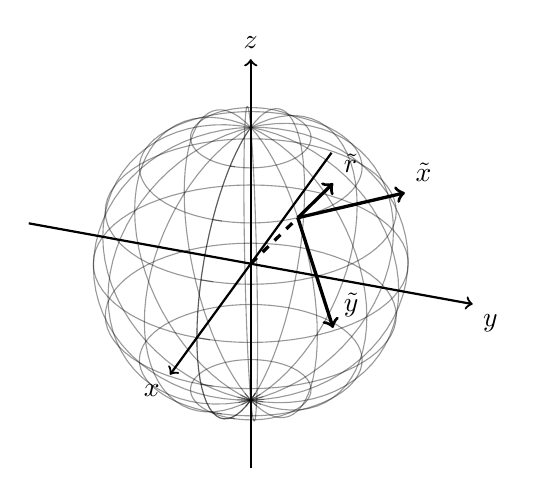
\begin{tikzpicture}    
    % Set up the 3D plot environment
    \tdplotsetmaincoords{60}{110}
    \begin{scope}[tdplot_main_coords]

            % Draw the main coordinate axes
            \draw[thick, ->] (-3,0,0) -- (3,0,0) node[anchor=north east] {$x$};
            \draw[thick, ->] (0,-3,0) -- (0,3,0) node[anchor=north west] {$y$};
            \draw[thick, ->] (0,0,-3) -- (0,0,3) node[anchor=south] {$z$};

            % Draw axes of r tilde, y tilde, x tilde
            \draw[very thick, dashed] (0, 0, 0) -- ({2*sin(45)*cos(45)},{2*sin(45)*sin(45)},{2*cos(45)});
            \draw[very thick, ->] ({2*sin(45)*cos(45)},{2*sin(45)*sin(45)},{2*cos(45)}) -- ({3.5*sin(45)*cos(45)},{3.5*sin(45)*sin(45)},{3.5*cos(45)}) node[anchor=south west] {$\tilde r$};
            \draw[very thick, ->] ({2*sin(45)*cos(45)},{2*sin(45)*sin(45)},{2*cos(45)}) -- ({2*sin(45)*cos(45) + 1.5*cos(45)*cos(45)},{2*sin(45)*sin(45) + 1.5*cos(45)*sin(45)},{2*cos(45) - 1.5*sin(45)}) node[anchor=south west] {$\tilde y$};
            \draw[very thick, ->] ({2*sin(45)*cos(45)},{2*sin(45)*sin(45)},{2*cos(45)}) -- ({2*sin(45)*cos(45) - 1.5*sin(45)},{2*sin(45)*sin(45) +1.5*cos(45)},{2*cos(45)}) node[anchor=south west] {$\tilde x$};
                    % Draw parametric surface for a sphere with great arcs at 22.5 degree intervals
        \foreach \u in {0,22.5,...,180} { % Latitude intervals of 22.5 degrees
        \foreach \v in {0,5,...,360} { % Small steps for smoothness in longitude
            % Calculate coordinates for each point on the surface
            \pgfmathsetmacro\x{2*sin(\u)*cos(\v)}
            \pgfmathsetmacro\y{2*sin(\u)*sin(\v)}
            \pgfmathsetmacro\z{2*cos(\u)}

            % Calculate next point in the longitude direction for smoothness
            \pgfmathsetmacro\lx{2*sin(\u)*cos(\v+5)}
            \pgfmathsetmacro\ly{2*sin(\u)*sin(\v+5)}
            \pgfmathsetmacro\lz{2*cos(\u)}

            % Draw line segments along latitude to form great arcs
            \draw[opacity=0.4] (\x,\y,\z) -- (\lx,\ly,\lz);
        }
    }

    \foreach \v in {0,22.5,...,360} { % Longitude intervals of 22.5 degrees
        \foreach \u in {0,5,...,180} { % Small steps for smoothness in latitude
            % Calculate coordinates for each point on the surface
            \pgfmathsetmacro\x{2*sin(\u)*cos(\v)}
            \pgfmathsetmacro\y{2*sin(\u)*sin(\v)}
            \pgfmathsetmacro\z{2*cos(\u)}

            % Calculate next point in the latitude direction for smoothness
            \pgfmathsetmacro\nx{2*sin(\u+5)*cos(\v)}
            \pgfmathsetmacro\ny{2*sin(\u+5)*sin(\v)}
            \pgfmathsetmacro\nz{2*cos(\u+5)}

            % Draw line segments along longitude to form great arcs
            \draw[opacity=0.4] (\x,\y,\z) -- (\nx,\ny,\nz);
        }
    }
            

    \end{scope}
\end{tikzpicture}    

    \caption{
        $(\tilde r, \tilde y, \tilde x)$ coordinates defined for a point on the unit sphere. These act as ordinary cartesian coordinates but rotated such that, at the associated point on $S^2$, $\hat{\tilde r}$ points straight out of the unit sphere, $\hat{\tilde y}$ is parallel to the great arc with constant $\phi$ and $\hat{\tilde x}$ is parallel to the great arc with constant $\theta$. These coordinates are used to define the shear and convergence in terms of the lensing potential.
        }
    \label{fig:tildecoords}
\end{figure}

Note that there it isn't obvious whether to define these coordinates at the point where the lensed light hits $S^2$ or the unlensed light hits $S^2$. We will assume that lensing effects are sufficiently weak that either definition works. We can then express the tilde coordinates in terms of spherical coordinates either by applying a rotation matrix or by calculating the $r, \theta, \phi$ derivatives of $(x,y,z)$ coordinates at $(r_0, \theta_0, \phi_0)$ to find $\hat{\tilde{\mathbf r}}$, $\hat{\tilde{\boldsymbol{\theta}}}$, and $\hat{\tilde{\boldsymbol{\phi}}}$ and then take inner products. Regardless, we find
\begin{align}
    \tilde r &= r\sin\theta\cos\phi\sin\theta_0\cos\phi_0+r\sin\theta\sin\phi\sin\theta_0\sin\phi_0+r\cos\theta\cos\theta_0,\\
    \tilde y &= r\sin\theta\cos\phi\cos\theta_0\cos\phi_0+r\sin\theta\sin\phi\cos\theta_0\sin\phi_0-r\cos\theta\sin\theta_0,\\
    \tilde x &= -r\sin\theta\cos\phi\sin\phi_0+r\sin\theta\sin\phi\cos\phi_0.
\end{align}
This gives derivatives
\begin{align*}
    \frac{\partial}{\partial \theta} = & \left( r \cos \theta \cos \phi \sin \theta_0 \cos \phi_0 + r \cos \theta \sin \phi \sin \theta_0 \sin \phi_0 - r \sin \theta \cos \theta_0 \right) \frac{\partial}{\partial \tilde{r}} \\
    & + \left( r \cos \theta \cos \phi \cos \theta_0 \cos \phi_0 + r \cos \theta \sin \phi \cos \theta_0 \sin \phi_0 + r \sin \theta \sin \theta_0 \right) \frac{\partial}{\partial \tilde{y}} \\
    & + \left( -r \cos \theta \cos \phi \sin \phi_0 + r \cos \theta \sin \phi \cos \phi_0 \right) \frac{\partial}{\partial \tilde{x}}.\\
    \frac{\partial}{\partial \phi} = & \left( -r \sin \theta \sin \phi \sin \theta_0 \cos \phi_0 + r \sin \theta \cos \phi \sin \theta_0 \sin \phi_0 \right) \frac{\partial}{\partial \tilde{r}} \\
& + \left( -r \sin \theta \sin \phi \cos \theta_0 \cos \phi_0 + r \sin \theta \cos \phi \cos \theta_0 \sin \phi_0 \right) \frac{\partial}{\partial \tilde{y}} \\
& + \left( r \sin \theta \sin \phi \sin \phi_0 + r \sin \theta \cos \phi \cos \phi_0 \right) \frac{\partial}{\partial \tilde{x}}.
\end{align*}
Evaluated at our point of interest we obtain $\partial_\theta=\partial_{\tilde y}$ and $\partial_\phi=\sin\theta_0\partial_{\tilde x}$. The second order derivatives can then be obtained using the first order derivatives. We can immediately evaluate them at the point to get
\begin{align*}
    \partial_\phi^2|_{(r_0,\theta_0,\phi_0)}&=-\sin^2\theta_0\partial_{\tilde r}-\sin\theta_0\cos\theta_0\partial_{\tilde y}+\sin^2\theta_0\partial^2_{\tilde x},\\
    \partial_\theta\partial_\phi|_{(r_0,\theta_0,\phi_0)}&=\cos\theta_0\partial_{\tilde x}+\sin\theta_0\partial_{\tilde x}\partial_{\tilde y},\\
    \partial_\theta^2|_{(r_0,\theta_0,\phi_0)}&=-\partial_{\tilde r}+\partial^2_{\tilde y}.
\end{align*}
Thus, at $(r_0, \theta_0, \phi_0)$,
\begin{gather*}
    \frac{1}{2}\eth_1(\eth_0\psi) = \frac{1}{2}\sin\theta(\partial_\theta+\frac{i}{\sin\theta}\partial_\phi)(\frac{1}{\sin\theta}(\partial_\theta+\frac{1}{\sin\theta}\partial_\phi))\\
    =\frac{\partial^2 \psi}{\partial \theta^2} - \frac{\cos\theta}{\sin\theta} \frac{\partial \psi}{\partial \theta} + \frac{2 i}{\sin\theta} \frac{\partial^2 \psi}{\partial \theta \partial \phi} - \frac{1}{\sin^2\theta} \frac{\partial^2 \psi}{\partial \phi^2} - 2 i \frac{\cos\theta}{\sin^2\theta} \frac{\partial \psi}{\partial \phi}\\
    =\frac{1}{2}(\partial_{\tilde y}^2 - \partial_{\tilde x}^2 + 2i\partial_{\tilde x}\partial_{\tilde y})\psi
    =\gamma_1 + i\gamma_2 = \gamma,
\end{gather*}
as required.

% \section{Fisher matrices raw data}

% Bispectra Fisher matrices:\\
% \begin{gather*}
% F^B_{\psi_c} =
% \begin{pmatrix}
% 4\times 10^{-3} & 6\times 10^{-4} & -6\times 10^{-3} & -9\times 10^{-3} & 1\times 10^{-4} & -4\times 10^{-3} & -1\times 10^{-3}\\
% 6\times 10^{-4} & 1\times 10^{-4} & -1\times 10^{-3} & -2\times 10^{-3} & 2\times 10^{-5} & -6\times 10^{-4} & -2\times 10^{-4}\\
% -6\times 10^{-3} & -1\times 10^{-3} & 1\times 10^{-2} & 1\times 10^{-2} & -2\times 10^{-4} & 6\times 10^{-3} & 2\times 10^{-3}\\
% -9\times 10^{-3} & -2\times 10^{-3} & 1\times 10^{-2} & 2\times 10^{-2} & -2\times 10^{-4} & 8\times 10^{-3} & 3\times 10^{-3}\\
% 1\times 10^{-4} & 2\times 10^{-5} & -2\times 10^{-4} & -2\times 10^{-4} & 3\times 10^{-6} & -1\times 10^{-4} & -3\times 10^{-5}\\
% -4\times 10^{-3} & -6\times 10^{-4} & 6\times 10^{-3} & 8\times 10^{-3} & -1\times 10^{-4} & 4\times 10^{-3} & 1\times 10^{-3}\\
% -1\times 10^{-3} & -2\times 10^{-4} & 2\times 10^{-3} & 3\times 10^{-3} & -3\times 10^{-5} & 1\times 10^{-3} & 4\times 10^{-4}
% \end{pmatrix},
% \\
% F^B_{\psi_s} =
% \begin{pmatrix}
% 3\times 10^{-1} & 4\times 10^{-2} & -3\times 10^{-1} & -1\times 10^{-1} & 5\times 10^{-3} & -1\times 10^{-1} & -1\times 10^{-1}\\
% 4\times 10^{-2} & 4\times 10^{-3} & -3\times 10^{-2} & -2\times 10^{-2} & 5\times 10^{-4} & -1\times 10^{-2} & -1\times 10^{-2}\\
% -3\times 10^{-1} & -3\times 10^{-2} & 2\times 10^{-1} & 1\times 10^{-1} & -3\times 10^{-3} & 1\times 10^{-1} & 1\times 10^{-1}\\
% -1\times 10^{-1} & -2\times 10^{-2} & 1\times 10^{-1} & 7\times 10^{-2} & -2\times 10^{-3} & 6\times 10^{-2} & 5\times 10^{-2}\\
% 5\times 10^{-3} & 5\times 10^{-4} & -3\times 10^{-3} & -2\times 10^{-3} & 6\times 10^{-5} & -2\times 10^{-3} & -2\times 10^{-3}\\
% -1\times 10^{-1} & -1\times 10^{-2} & 1\times 10^{-1} & 6\times 10^{-2} & -2\times 10^{-3} & 6\times 10^{-2} & 5\times 10^{-2}\\
% -1\times 10^{-1} & -1\times 10^{-2} & 1\times 10^{-1} & 5\times 10^{-2} & -2\times 10^{-3} & 5\times 10^{-2} & 5\times 10^{-2}
% \end{pmatrix},
% \\
% F^B_{\psi_{s + c}} =
% \begin{pmatrix}
% 4\times 10^{-1} & 4\times 10^{-2} & -3\times 10^{-1} & -2\times 10^{-1} & 5\times 10^{-3} & -2\times 10^{-1} & -1\times 10^{-1}\\
% 4\times 10^{-2} & 4\times 10^{-3} & -3\times 10^{-2} & -2\times 10^{-2} & 6\times 10^{-4} & -2\times 10^{-2} & -1\times 10^{-2}\\
% -3\times 10^{-1} & -3\times 10^{-2} & 2\times 10^{-1} & 2\times 10^{-1} & -4\times 10^{-3} & 1\times 10^{-1} & 1\times 10^{-1}\\
% -2\times 10^{-1} & -2\times 10^{-2} & 2\times 10^{-1} & 1\times 10^{-1} & -3\times 10^{-3} & 8\times 10^{-2} & 7\times 10^{-2}\\
% 5\times 10^{-3} & 6\times 10^{-4} & -4\times 10^{-3} & -3\times 10^{-3} & 7\times 10^{-5} & -2\times 10^{-3} & -2\times 10^{-3}\\
% -2\times 10^{-1} & -2\times 10^{-2} & 1\times 10^{-1} & 8\times 10^{-2} & -2\times 10^{-3} & 7\times 10^{-2} & 6\times 10^{-2}\\
% -1\times 10^{-1} & -1\times 10^{-2} & 1\times 10^{-1} & 7\times 10^{-2} & -2\times 10^{-3} & 6\times 10^{-2} & 5\times 10^{-2}
% \end{pmatrix}.
% \end{gather*}

% Powerspectra Fisher matrices:
% \begin{gather*}
% F^P_{\psi_c} =
% \begin{pmatrix}
% 2\times 10^{-2} & 4\times 10^{-3} & -4\times 10^{-2} & 8\times 10^{-3} & 9\times 10^{-4} & -3\times 10^{-2} & -1\times 10^{-2}\\
% 4\times 10^{-3} & 1\times 10^{-3} & -9\times 10^{-3} & -6\times 10^{-4} & 2\times 10^{-4} & -5\times 10^{-3} & -2\times 10^{-3}\\
% -4\times 10^{-2} & -9\times 10^{-3} & 8\times 10^{-2} & -9\times 10^{-3} & -2\times 10^{-3} & 6\times 10^{-2} & 2\times 10^{-2}\\
% 8\times 10^{-3} & -6\times 10^{-4} & -9\times 10^{-3} & 2\times 10^{-2} & 3\times 10^{-4} & -1\times 10^{-2} & -4\times 10^{-3}\\
% 9\times 10^{-4} & 2\times 10^{-4} & -2\times 10^{-3} & 3\times 10^{-4} & 3\times 10^{-5} & -1\times 10^{-3} & -4\times 10^{-4}\\
% -3\times 10^{-2} & -5\times 10^{-3} & 6\times 10^{-2} & -1\times 10^{-2} & -1\times 10^{-3} & 4\times 10^{-2} & 2\times 10^{-2}\\
% -1\times 10^{-2} & -2\times 10^{-3} & 2\times 10^{-2} & -4\times 10^{-3} & -4\times 10^{-4} & 2\times 10^{-2} & 6\times 10^{-3}
% \end{pmatrix},
% \\
% F^P_{\psi_s} =
% \begin{pmatrix}
% 2\times 10^{-1} & 1\times 10^{-2} & -1\times 10^{-1} & -3\times 10^{-2} & 2\times 10^{-3} & -6\times 10^{-2} & -7\times 10^{-2}\\
% 1\times 10^{-2} & 1\times 10^{-3} & -9\times 10^{-3} & -3\times 10^{-3} & 2\times 10^{-4} & -5\times 10^{-3} & -6\times 10^{-3}\\
% -1\times 10^{-1} & -9\times 10^{-3} & 7\times 10^{-2} & 2\times 10^{-2} & -1\times 10^{-3} & 4\times 10^{-2} & 4\times 10^{-2}\\
% -3\times 10^{-2} & -3\times 10^{-3} & 2\times 10^{-2} & 9\times 10^{-3} & -4\times 10^{-4} & 1\times 10^{-2} & 1\times 10^{-2}\\
% 2\times 10^{-3} & 2\times 10^{-4} & -1\times 10^{-3} & -4\times 10^{-4} & 3\times 10^{-5} & -7\times 10^{-4} & -8\times 10^{-4}\\
% -6\times 10^{-2} & -5\times 10^{-3} & 4\times 10^{-2} & 1\times 10^{-2} & -7\times 10^{-4} & 2\times 10^{-2} & 2\times 10^{-2}\\
% -7\times 10^{-2} & -6\times 10^{-3} & 4\times 10^{-2} & 1\times 10^{-2} & -8\times 10^{-4} & 2\times 10^{-2} & 3\times 10^{-2}
% \end{pmatrix},
% \\
% F^P_{\psi_{s+c}} =
% \begin{pmatrix}
% 9\times 10^{-2} & 9\times 10^{-3} & -7\times 10^{-2} & -1\times 10^{-2} & 1\times 10^{-3} & -4\times 10^{-2} & -4\times 10^{-2}\\
% 9\times 10^{-3} & 1\times 10^{-3} & -9\times 10^{-3} & -2\times 10^{-3} & 2\times 10^{-4} & -5\times 10^{-3} & -4\times 10^{-3}\\
% -7\times 10^{-2} & -9\times 10^{-3} & 7\times 10^{-2} & 8\times 10^{-3} & -1\times 10^{-3} & 5\times 10^{-2} & 3\times 10^{-2}\\
% -1\times 10^{-2} & -2\times 10^{-3} & 8\times 10^{-3} & 2\times 10^{-2} & -7\times 10^{-5} & -3\times 10^{-4} & 5\times 10^{-3}\\
% 1\times 10^{-3} & 2\times 10^{-4} & -1\times 10^{-3} & -7\times 10^{-5} & 3\times 10^{-5} & -9\times 10^{-4} & -6\times 10^{-4}\\
% -4\times 10^{-2} & -5\times 10^{-3} & 5\times 10^{-2} & -3\times 10^{-4} & -9\times 10^{-4} & 3\times 10^{-2} & 2\times 10^{-2}\\
% -4\times 10^{-2} & -4\times 10^{-3} & 3\times 10^{-2} & 5\times 10^{-3} & -6\times 10^{-4} & 2\times 10^{-2} & 2\times 10^{-2}
% \end{pmatrix}.
% \end{gather*}




\end{document}
